\chapter{Mutation-Based Fault Trace Generation for Transformer Architectures}
\label{chapter_frankenformer}

DEFault (Chapter~\ref{chapter_default}) demonstrates effective fault detection and diagnosis for FFNNs, CNNs, and RNNs, but it does not support attention-based architectures.
Chapter~\ref{chapter_attention} establishes a detailed taxonomy of faults specific to attention-based architectures, and Chapter~\ref{chapter_hessian} shows that Hessian-based analysis can reveal diagnostic signals missed by gradient-based methods in these models. Extending DEFault to transformers requires labeled fault data that links implementation-level faults to their observable behavioral effects.
Real-world fault data for transformers is scarce; therefore, we follow the strategy used in DEFault for classic DNNs and generate synthetic fault data through mutation. In this chapter, we introduce FrankenFormer, a fault injection framework for transformer architectures. FrankenFormer injects taxonomy-based faults into transformer components and characterizes their effects using internal diagnostic metrics and task-specific metrics.
Its primary output is a labeled dataset of fault traces of transformer models derived from clean and faulty fine-tuning runs.
We apply FrankenFormer to seven encoder and decoder models across nine tasks, producing 3{,}739 validated single-fault configurations. Each configuration contributes multiple clean and faulty runs.
The resulting labeled traces form the basis of an automated fault-diagnosis framework for transformers, presented in the next chapter.

The rest of this chapter is organized as follows.
Section~\ref{sec:frankenformer-introduction} introduces the chapter.
Section~\ref{sec:frankenformer-methodology} presents the methodology, including the fault injection framework, injection mechanism, and validation procedure.
Section~\ref{sec:mutation-analysis} reports the experimental setup, results, and analysis.
Section~\ref{sec:threats} discusses threats to validity.
Section~\ref{sec:related-work} reviews related work.
Section~\ref{sec:frankformer-summary} concludes the chapter.

\section{Introduction}
\label{sec:frankenformer-introduction}
Transformers are widely used across language, vision, and multimodal modeling.
Their effectiveness stems largely from the attention mechanism~\citep{vaswani2017attention}.
Although the attention mechanism addresses long-standing limitations of sequential models such as Recurrent Neural Networks (RNNs), its implementation through complex software stacks combining model code, optimized kernels, mixed-precision arithmetic, and task-specific data pipelines introduces reliability risks~\citep{zhang2020machine,ABNN_sigma,attentiondetails}. In particular, small implementation mistakes in attention logic, masking, or kernel integration can silently alter model behavior without triggering any explicit failures.

Several studies show that transformers can develop subtle internal anomalies~\cite{ABNN_sigma,attentionPlease,attentioncollapse,attentioncollapsecompress,miller2023attention}. For example, attention heads can degenerate or become redundant~\citep{michel2019sixteen,voita2019analyzing}. When multiple heads converge to produce similar attention patterns across the input, the model loses the representational diversity that multi-head attention is designed to provide.
Masks can be incorrectly applied, causing attention weights to drift toward padding tokens~\citep{dao2022flashattention,vaswani2017attention}.
Score computation can be numerically unstable, which affects gradient flow during fine-tuning~\citep{xiong2020layer,mosbach2021stability}.
These anomalies can corrupt internal representations while leaving end-task accuracy largely unchanged.

Prior work shows that pruning or freezing attention heads can preserve accuracy even when the model's internal behavior diverges considerably from its correct baseline~\citep{michel2019sixteen}. Separate work reports that silent and latent faults occur in Attention-based Neural Networks (ABNNs) at twice the rate observed in classic Deep Neural Networks (DNNs)~\citep{ABNN_sigma}, which underscores the scale of this problem.
In settings such as medical diagnosis, a model that passes standard accuracy benchmarks despite corrupted internal representations may still pose risks that accuracy-based evaluation does not capture.

Standard evaluation methods rely on measures such as accuracy, perplexity, or F1~\citep{wang2018glue}, but they can miss faults that alter internal signals without degrading task performance. For example, attention heads may collapse to near-uniform distributions while classification accuracy remains largely unchanged.
To link implementation-level faults to their behavioral effects in internal diagnostic metrics, we need execution traces with ground-truth fault labels. These labels must map specific implementation errors to shifts in metric distributions.

Establishing such connections is challenging because existing mutation frameworks do not target transformer-specific fault components. Techniques like DeepCrime, DeepMutation, and DeepMutation++ define operators for generic neural network components such as hyperparameter and activation functions~\citep{deepmetis,deepmutation++,deepcrime,deepmutation}, while hardware-oriented tools such as PyTorchFI\footnote{\url{https://github.com/DependableSystemsLab/pytorchfi}} inject low-level corruptions (e.g., bit-flips) rather than attention-level faults~\citep{pytorchfi}. Neither class of techniques covers transformer-specific phenomena such as masking logic, QKV projection errors, positional encoding faults, or KV cache mismanagement~\citep{ABNN_sigma}. As a result, no existing operator can, for example, inject a missing padding mask or a swapped query-key projection in a transformer model.
Prior techniques are therefore inadequate to produce fault labels at the granularity needed for attention-related fault diagnosis.

To address this gap, FrankenFormer injects implementation-level faults into transformer components and generates labeled fault traces from clean and faulty training runs. The framework draws on the taxonomy of attention-based neural network failures established in Chapter~\ref{chapter_attention} and extends it to six core transformer units: embeddings, multi-head self-attention, feed-forward networks, layer normalization, residual connections, and output projections (Figure~\ref{fig:fault-taxonomy}).
Across seven encoder and decoder models and nine tasks, FrankenFormer produces 3{,}739 validated single-fault configurations.
Our results show that encoder faults are more likely than decoder faults to produce detectable behavioral shifts. Many encoder faults that produce statistically significant shifts in internal behavior do not degrade end-task accuracy, indicating that accuracy-only evaluation misses faults visible in behavioral diagnostics.

FrankenFormer also produces a labeled fault-trace dataset that links each injected fault to its behavioral and task-level effects, providing ground-truth labels for downstream diagnosis. This chapter makes the following contributions:
\begin{itemize}[leftmargin=*, nosep]
    \item A fault injection framework based on our taxonomy, FrankenFormer, targeting six transformer components, twelve fault categories, and 45 root causes (40 for encoders, 45 for decoders) that represent realistic implementation errors.

    \item A validation procedure based on an internal-behavior criterion and an end-task performance criterion to classify fault outcomes.

    \item A publicly available fault-trace dataset spanning seven encoder and decoder architectures and nine downstream tasks.\footnote{Replication package: \url{https://github.com/SigmaJahan/frankenformer-mutation-testing}}
\end{itemize}

\begin{figure}[!htbp]
    \centering
    \resizebox{0.88\textwidth}{!}{
        \input{figures/frankformer/diagram}
    }
    \caption[Fault categories organized by transformer component.]{Overview of the fault categories organized by transformer component. Part~(a) shows faults at the transformer-block level; part~(b) zooms into the attention internals.}
    \label{fig:fault-taxonomy}
\end{figure}

\section{Methodology}
\label{sec:frankenformer-methodology}

FrankenFormer is a fault injection framework for transformer models. Given a pretrained model and a downstream task, the framework injects implementation-level faults into controlled components, performs matched clean and faulty training runs, and produces a dataset of metric trajectories with ground-truth configuration labels.
The framework builds on prior taxonomies of faults in attention-based neural networks~\citep{ABNN_sigma} and adapts techniques from mutation testing of deep neural networks~\citep{deepmutation++,deepcrime,deepmutation}, differential testing~\citep{Tian2017}, and behavioral invariance testing~\citep{chen2018metamorphic,ribeiro2020checklist}.

%==============================================================================
\subsection{Fault Model}
\label{subsec:fault-model}

The fault categories and variants are grounded in the ABNN taxonomy introduced in Chapter~\ref{chapter_attention}. We focus on realistic implementation errors, including configuration mistakes and silent numerical issues. Specifically, we select fault configurations that execute without explicit runtime errors and require behavioral or statistical observation for detection. We exclude explicit faults because conventional tests or runtime checks often detect them. We then translate this subset into a programmable fault model.

\paragraph{Transformer decomposition.}
We decompose each transformer block into six \emph{units} that match common implementation boundaries. For a standard transformer block~\citep{vaswani2017attention}:
\begin{align}
\mathbf{h} &= \mathrm{LayerNorm}\bigl(\mathbf{x} + \mathrm{MHA}(\mathbf{x})\bigr) \label{eq:attn-block}\\
\mathbf{y} &= \mathrm{LayerNorm}\bigl(\mathbf{h} + \mathrm{FFN}(\mathbf{h})\bigr) \label{eq:ffn-block}
\end{align}
where $\mathbf{x} \in \mathbb{R}^{n \times d}$ is an input sequence, MHA is multi-head self-attention, and FFN is a position-wise feed-forward network.
From this structure, we define six units: embeddings (input representations), multi-head self-attention, FFN, layer normalization, residual connections, and the output projection head.
The same unit boundaries apply under pre-norm variants; only the ordering of LayerNorm changes.
For each unit, we define one or more \emph{fault categories}, and each category contains several concrete \emph{variants} that mimic specific bug patterns.

\paragraph{Attention fault categories.}
Multi-head self-attention is both the most complex unit and a frequent source of faults in practice~\citep{ABNN_sigma,michel2019sixteen,voita2019analyzing}. We write self-attention as
\begin{equation}
\mathrm{Attention}(Q, K, V) = \mathrm{softmax}\!\left(\frac{QK^\top}{\sqrt{d_k}} + M\right)V
\label{eq:attention}
\end{equation}
where $Q, K, V$ are linear projections of the input, $d_k$ is the key dimension, and $M$ is an additive mask.
We treat each component of Equation~\ref{eq:attention} as a potential fault surface and group faults into seven categories following the ABNN taxonomy from Chapter~\ref{chapter_attention}. The first six apply to both encoders and decoders; the last is decoder-only.

\begin{itemize}

  \item \emph{Attention masking faults} corrupt the mask $M$. They represent missing padding masks, inverted mask logic, and incorrect reshaping of the mask tensor across batch and head dimensions. For decoder-only self-attention, this category also covers \emph{causal-mask violations} that allow attention to flow from position $i$ to future positions $j>i$ (i.e., future leakage), while still executing without runtime errors.

  \item \emph{QKV projection faults} corrupt the projection matrices $W^Q, W^K, W^V$. They represent shared or swapped projections, zero-initialized projections, and frozen parameters that prevent individual heads from learning distinct attention patterns~\citep{michel2019sixteen,voita2019analyzing}.

  \item \emph{Score computation faults} corrupt the scaling and dropout around the attention scores. They represent missing $1/\sqrt{d_k}$ scaling, misplaced dropout, and unsafe mixed-precision conversions that affect numerical stability.

  \item \emph{Positional encoding faults} corrupt positional information through off-by-one errors, truncation beyond the supported sequence length, or complete omission of positional embeddings.

  \item \emph{Kernel faults} stem from the misconfiguration of attention kernels. They represent mismatched dropout probabilities between training configuration and kernel invocation, data type or layout constraints that trigger silent backend fallbacks, and forced use of non-optimized kernels, which change runtime behavior without necessarily changing model structure.

  \item \emph{Attention variant faults} represent the selection of a wrong attention variant, such as single-head instead of multi-head attention, or applying causal masking in a bidirectional encoder (encoder-only).

  \item \emph{KV cache faults} target key-value cache management in autoregressive decoders. They represent stale caches (failure to update $K/V$ for some layers or steps), off-by-one indexing (writing or reading at shifted positions), truncated caches for long sequences, and cross-request cache leaks (caches not cleared between prompts). These faults preserve generation capability but make the decoded content non-equivalent to full-recompute decoding~\citep{adnan2024keyformer}.
\end{itemize}

\paragraph{Other fault categories.}
Each remaining unit has a single fault category.

\begin{itemize}
  \item \emph{Input embedding faults} corrupt token and type embeddings (i.e., segment identifiers used in models such as BERT) by zeroing subsets, swapping embeddings, or scaling segment embeddings.
  \item \emph{Feed-forward Network (FFN) faults} alter hidden-layer characteristics by scaling weights, permanently dropping neurons, or replacing the nonlinearity (e.g., $\mathrm{GELU} \rightarrow \mathrm{ReLU}$).
  \item \emph{Layer normalization faults} modify LayerNorm parameters by scaling or zeroing the learned scale parameter $\gamma$, shifting the learned bias parameter $\beta$, or misconfiguring the numerical stability term $\epsilon$, which is known to affect optimization and gradient flow~\citep{xiong2020layer,mosbach2021stability}.
  \item \emph{Residual connection faults} break skip connections by removing them, scaling the residual path, or injecting noise into the skip branch.
  \item \emph{Output projection faults} corrupt prediction heads by scaling logits, zeroing rows corresponding to selected output classes, or reinitializing the output projection.
\end{itemize}

Figure~\ref{fig:full-fault-taxonomy} presents the complete fault taxonomy used by FrankenFormer. The seven attention-specific fault categories and their 25 root causes are derived from the attention fault taxonomy established in Chapter~\ref{chapter_attention}~\cite{attention_taxonomy}. The remaining five categories (Input/Embedding, Layer Normalization, Feed-Forward Network, Residual, and Output) and their 20 root causes are derived from the DNN fault taxonomy by~\citet{faulttaxonomy} and the mutation operators defined by~\citet{deepcrime}. Each root cause name identifies the fundamental mechanism or parameter that is faulty (e.g., activation function, dropout rate, weight scaling) rather than a specific corrective action. The 12 fault categories collectively define 45 root causes across encoder and decoder architectures (40 for encoders, 45 for decoders).

\begin{figure}[!htbp]
\centering
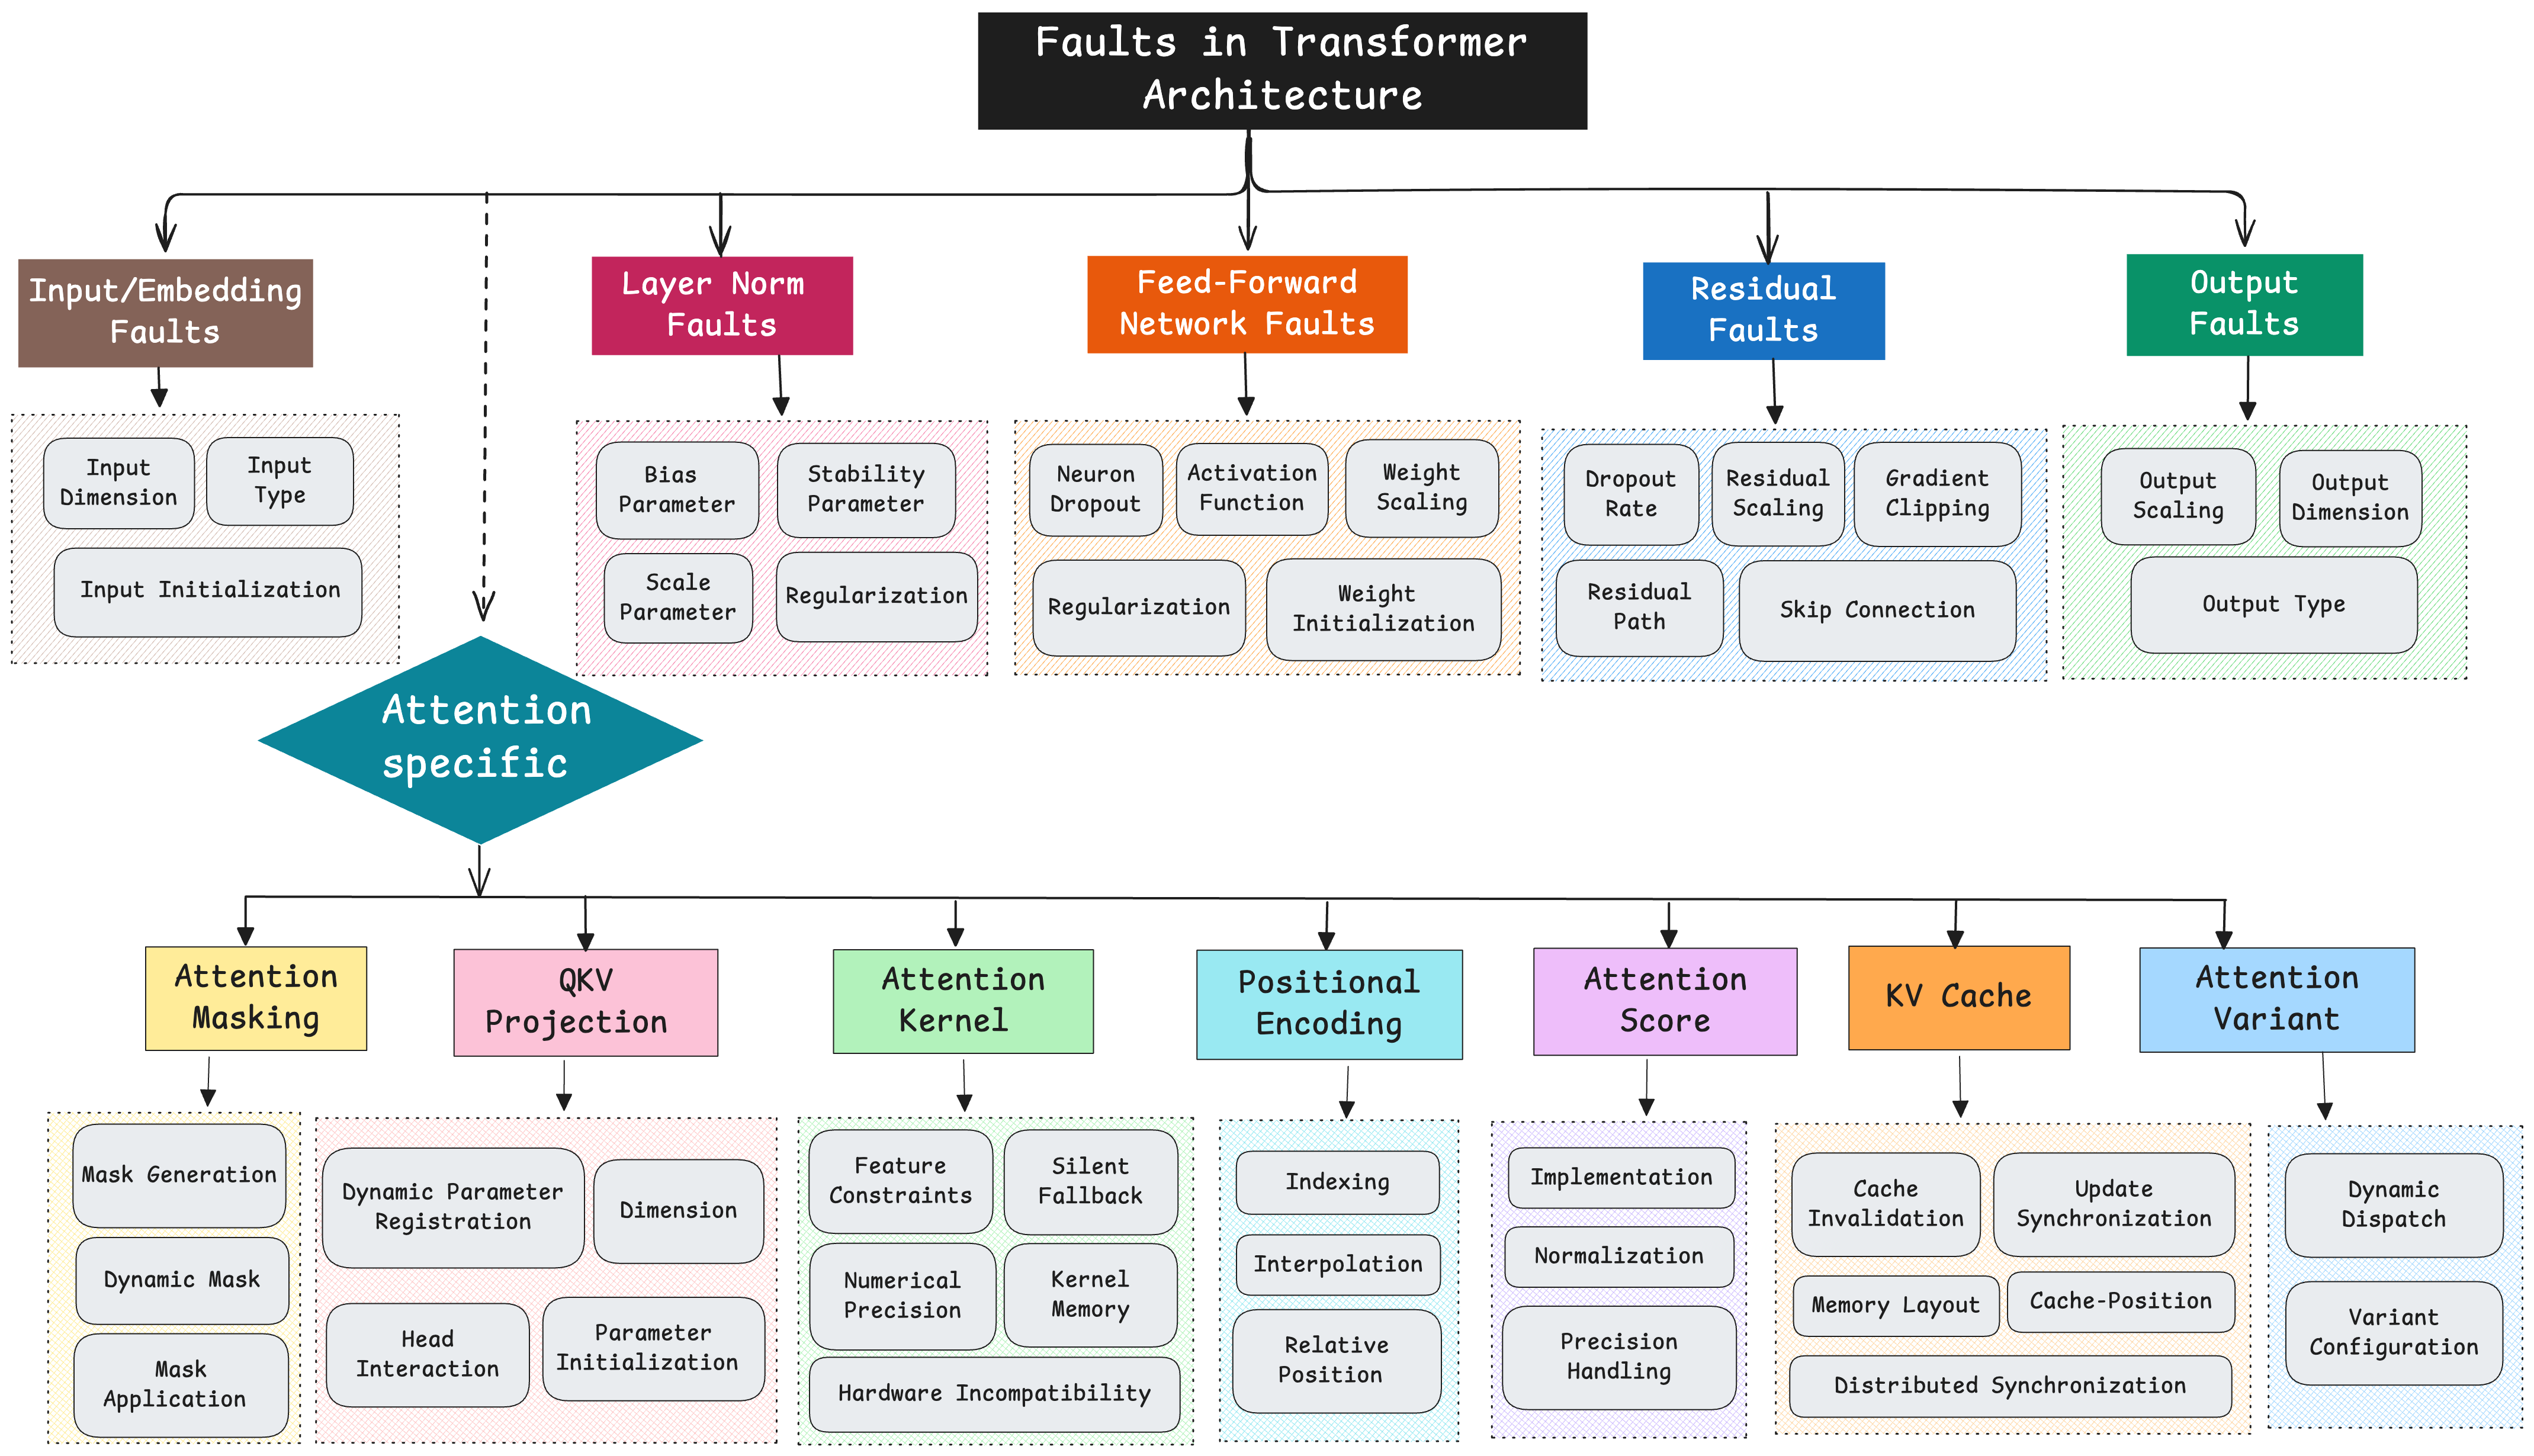
\includegraphics[width=\textwidth]{taxonomy-chapter-7-8.png}
\caption[Complete fault taxonomy for transformer architectures.]{Complete fault taxonomy for transformer architectures. The seven attention-specific categories (bottom) and their 25 root causes are derived from the attention fault taxonomy (Chapter~\ref{chapter_attention}). The five non-attention categories (top) and their 20 root causes are derived from prior DNN fault taxonomies and DeepCrime mutation operators.}
\label{fig:full-fault-taxonomy}
\end{figure}

Table~\ref{tab:fault-taxonomy} summarizes the units, fault categories, representative variants, expected impacts, and the metrics sensitive to each impact type.

\begin{table}[!htbp]
\caption{Fault categories organized by transformer unit.}
\label{tab:fault-taxonomy}
\centering
\scriptsize
\renewcommand{\arraystretch}{1.10}
\setlength{\tabcolsep}{4pt}
\begin{tabularx}{\linewidth}{@{}
  l
  >{\raggedright\arraybackslash}X
  >{\raggedright\arraybackslash}X
  >{\raggedright\arraybackslash}X @{}}
\toprule
\textbf{Fault category} & \textbf{Representative variants} & \textbf{Expected impact} & \textbf{Relevant metrics} \\
\midrule
\addlinespace[0.2ex]
\multicolumn{4}{c}{\textit{--- Embedding ---}} \\
\addlinespace[0.2ex]
Input Embedding Faults &
Zero a token subset; swap embedding pairs; scale type embeddings &
Corrupted input representations \citep{bosio2024impact} &
Embedding norms, representation shift \citep{kornblith2019similarity} \\
\addlinespace[0.3ex]
\cmidrule(lr){1-4}
\addlinespace[0.2ex]
\multicolumn{4}{c}{\textit{--- Multi-Head Attention ---}} \\
\addlinespace[0.2ex]
Attention Masking Faults &
Zero the mask (attend to padding); invert the mask; reshape incorrectly across batch/heads &
Attention to padding or masked tokens \citep{dao2022flashattention,liu2024lost} &
Padding attention mass (Eq.~\ref{eq:padmass}), masked-region leakage; future leakage mass (decoder, Eq.~\ref{eq:futuremass}) \citep{vaswani2017attention,dao2022flashattention} \\
QKV Projection Faults &
Zero $Q/K/V$ projections; swap $Q\!\leftrightarrow\! K$; tie head weights; freeze gradients &
Degenerate or frozen attention heads \citep{michel2019sixteen,voita2019analyzing,bhojanapalli2020lowrank} &
Inter-head cosine similarity, QKV gradient norms \citep{clark2019does} \\
Score Computation Faults &
Omit $1/\!\sqrt{d_k}$ scaling; apply dropout before softmax; cast unsafely to float16 &
Miscalibrated or unstable attention scores \citep{dao2022flashattention,attentioncollapse,miller2023attention} &
Attention entropy, score mean \& variance \citep{clark2019does} \\
Positional Encoding Faults &
Omit positional embeddings; shift position indices; truncate positions beyond supported length &
Corrupted or inconsistent position information \citep{dufter-etal-2022-position,sinha-etal-2022-curious,kazemnejad2023impact} &
Positional sensitivity, representation drift \citep{sinha-etal-2022-curious,kiyono-etal-2021-shape,kornblith2019similarity} \\
Kernel Faults &
Force a slow backend; trigger fallback via data type or layout mismatch; use mismatched dropout probabilities &
Silent kernel fallback or numerical differences \citep{dao2022flashattention,liang2025attnchecker} &
Step duration, peak memory allocation~\cite{nvidia2021dlprof,chakrabarti2012cuda} \\
Attention Variant Faults &
Replace multi-head with single-head attention; apply causal mask in encoder (encoder-only) &
Reduced capacity or incorrect masking pattern \citep{michel2019sixteen,sandoval2025even} &
Head utilization, attention rank~\cite{michel2019sixteen,voita2019analyzing}\\
KV Cache Faults$^{\dagger}$ &
Use a stale cache; shift indices by one; truncate the cache; leak cache across requests &
Divergence between cached and fully recomputed hidden states; cross-request context leakage \citep{zhang2024layer,jiang2025foundation} &
Cache-vs-recompute hidden-state cosine similarity, next-token prediction divergence~\cite{zhang2024layer,jiang2025foundation} \\
\addlinespace[0.3ex]
\cmidrule(lr){1-4}
\addlinespace[0.2ex]
\multicolumn{4}{c}{\textit{--- Feed-Forward Network ---}} \\
\addlinespace[0.2ex]
FFN Faults &
Scale FFN weights; permanently drop neurons; change the activation function &
Altered layer characteristics and sparsity \citep{zhang2024transformerdoctor} &
FFN output norms, active neuron fraction~\cite{zhang2024transformerdoctor} \\
\addlinespace[0.3ex]
\cmidrule(lr){1-4}
\addlinespace[0.2ex]
\multicolumn{4}{c}{\textit{--- Layer Normalization ---}} \\
\addlinespace[0.2ex]
Layer Normalization Faults &
Scale or zero the scale parameter $\gamma$; shift the bias parameter $\beta$; change $\epsilon$ &
Mis-normalized activations \citep{xiong2020layer,mosbach2021stability} &
Activation mean/variance, $\|\gamma\|_2$ \citep{wortsman2024small} \\
\addlinespace[0.3ex]
\cmidrule(lr){1-4}
\addlinespace[0.2ex]
\multicolumn{4}{c}{\textit{--- Residual Connection ---}} \\
\addlinespace[0.2ex]
Residual Connection Faults &
Remove the skip connection; scale the residual branch; inject Gaussian noise &
Broken or noisy information flow \citep{vaswani2017attention,dong2021attention} &
Residual stream cosine similarity \citep{naitsaada2024mind} \\
\addlinespace[0.3ex]
\cmidrule(lr){1-4}
\addlinespace[0.2ex]
\multicolumn{4}{c}{\textit{--- Output ---}} \\
\addlinespace[0.2ex]
Output Projection Faults &
Scale logits; zero rows for selected output classes; reinitialize the output projection &
Corrupted output distribution and calibration \citep{bosio2024impact} &
Logit entropy, calibration error \citep{guo2017calibration} \\
\bottomrule
\end{tabularx}
\smallskip\\
{\scriptsize $^{\dagger}$Decoder-only category.}
\end{table}

\begin{figure}[!htbp]
    \centering
    \includegraphics[width=0.95\textwidth]{figures/frankformer/workflow.png}
    \caption{Workflow of FrankenFormer.}
    \label{fig:methodology-workflow}
\end{figure}

\subsection{Injection Mechanism}
\label{subsec:injection}

We denote the clean model parameters by $\theta$ and the injected mutant by $\theta'$. Each injected fault is specified by a configuration $\mathcal{C} = (m, t, u, f, v, \ell, \sigma)$, and we evaluate $\theta$ and $\theta'$ under the same random seeds and an identical fine-tuning pipeline to isolate the causal effect of $\mathcal{C}$.
\begin{algorithm}[!htbp]
\caption{Fault injection and validation pipeline (steps correspond to Figure~\ref{fig:methodology-workflow})}
\label{alg:injection}
\begin{algorithmic}[1]
\Require Model $\theta$, fault configuration $\mathcal{C}$, seeds $\mathcal{S}$, metrics $\mathcal{M}$
\Ensure Validation status, feature vector $\mathbf{x}$

\Statex \hfill\textit{--- Step~\textcircled{\scriptsize 1}: Input ---}
\State Receive model $\theta$ and benchmark dataset (task $t$ from $\mathcal{C}$)

\Statex \hfill\textit{--- Step~\textcircled{\scriptsize 2}: Fault Injection ---}
\State $\theta' \gets \text{Inject}(\theta, \mathcal{C})$ \Comment{Create mutant from fault taxonomy}
\State $v_{\text{struct}} \gets \text{VerifyStructuralIntegrity}(\theta, \theta', \mathcal{C})$ \Comment{Confirm targeted modification only}

\Statex \hfill\textit{--- Step~\textcircled{\scriptsize 3}: Paired Training ---}
\State $R_{\text{clean}} \gets \emptyset$, $R_{\text{faulty}} \gets \emptyset$ \Comment{Sets of per-seed metric trajectories}
\For{each seed $s \in \mathcal{S}$}
    \State $r_c \gets \text{TrainAndEvaluate}(\theta, s)$ \Comment{Clean run}
    \State $R_{\text{clean}} \gets R_{\text{clean}} \cup \{r_c\}$
    \State $r_f \gets \text{TrainAndEvaluate}(\theta', s)$ \Comment{Faulty run, same seed}
    \State $R_{\text{faulty}} \gets R_{\text{faulty}} \cup \{r_f\}$
\EndFor

\Statex \hfill\textit{--- Step~\textcircled{\scriptsize 4}: Metric Collection ---}
\State $\Delta \gets \text{ComputeDeltas}(R_{\text{clean}}, R_{\text{faulty}}, \mathcal{M})$ \Comment{Signed differences, normalized}

\Statex \hfill\textit{--- Step~\textcircled{\scriptsize 5}: Behavioral Validation ---}
\State $v_{\text{beh}} \gets \text{InternalBehaviorCriterion}(\Delta)$ \Comment{Permutation test, $p \leq 0.05$}
\If{$v_{\text{beh}} = 0$}
    \State Discard configuration \Comment{No statistically significant change}
\EndIf

\Statex \hfill\textit{--- Step~\textcircled{\scriptsize 6}: Outcome Classification ---}
\State $v_{\text{task}} \gets \text{EndTaskCriterion}(R_{\text{clean}}, R_{\text{faulty}})$ \Comment{Accuracy or perplexity threshold}
\State $\mathbf{x} \gets \text{Aggregate}(R_{\text{faulty}}, \mathcal{M})$
\State \Return $(v_{\text{struct}},\; v_{\text{beh}},\; v_{\text{task}}), \;\mathbf{x}$ \Comment{Finalize trace with fault label}
\end{algorithmic}
\end{algorithm}

\paragraph{Fault configurations.}

A fault configuration $\mathcal{C}$ specifies:
\begin{description}[leftmargin=1.6em,style=nextline,noitemsep]
  \item[$m$] model architecture (encoder or decoder checkpoint)
  \item[$t$] downstream task / dataset
  \item[$u$] target unit (Embedding, MHA, FFN, LayerNorm, Residual, Output)
  \item[$f$] fault category
  \item[$v$] fault variant within category
  \item[$\ell$] affected layer indices, $\ell \subseteq \{1,\dots,L\}$ where $L$ is the number of transformer blocks (typically a singleton; multi-site injection is not used in this study)
  \item[$\sigma$] severity level, $\sigma \in \{\mathrm{low}, \mathrm{medium}, \mathrm{high}\}$
\end{description}
The severity level controls the magnitude of perturbation for numeric variants, such as scaling factors and dropout rates. For non-numeric or discrete variants, severity maps to a discrete intensity parameter (e.g., visibility ratio in causal-mask breaking). For example, $\mathcal{C} = (\text{BERT-base},\; \text{SST-2 (Stanford Sentiment Treebank)},\; \text{MHA},\; \text{Masking},\; \text{ZeroMask},\; \ell=\{7\},\; \sigma=\text{high})$ indicates \emph{zeroing} the attention mask at layer~7 during fine-tuning on SST-2.

\paragraph{Static vs dynamic faults.}
Transformer faults affect either stored parameters or runtime computations, which requires two distinct injection mechanisms~\citep{pytorchfi,deepcrime}. We distinguish these two patterns (see Figure~\ref{fig:injection-code-panels}).

\emph{Static faults} modify parameter tensors at rest, before forward execution.
For example, an FFN weight-scaling fault multiplies selected weight matrices by a scalar:
\begin{equation}
\theta'_i =
\begin{cases}
\alpha \cdot \theta_i & \text{if } i \in \mathrm{params}(u,\ell),\\[0.2ex]
\theta_i & \text{otherwise}
\end{cases}
\label{eq:static-fault}
\end{equation}
where $\mathrm{params}(u,\ell)$ selects parameters of unit $u$ in layers $\ell$.
Static faults include embedding corruption, parameter scaling, permanent neuron dropout, and LayerNorm parameter changes.

\emph{Dynamic faults} modify the forward computation path through wrappers or hooks at selected module call sites.
For example, a mask-zeroing fault intercepts the attention call and replaces the mask $M$ by zeros:
\begin{equation}
\texttt{forward}'(x, M) = \texttt{forward}(x, \mathbf{0}_{|M|})
\label{eq:dynamic-fault}
\end{equation}
where $\mathbf{0}_{|M|}$ denotes a zero tensor of the same shape as the original mask $M$.
Dynamic faults include mask manipulation, Q/K swapping, removal of score scaling, and forced kernel selection. In both cases, the transformer architecture is unchanged. Only the targeted computation or parameter values are modified.

\paragraph{Decoder causality constraint.}
Decoder-only self-attention is causal by construction: the clean model enforces that token position $i$ cannot attend to future positions $j>i$. Therefore, any injected fault representing a \emph{causal violation} (e.g., ``wrong masking layout'' or ``broken causal mask'') must be implemented by \emph{removing or weakening} this constraint (allowing future attention), rather than by adding an additional causal mask. Specifically, we inject causal violations by replacing a configurable fraction of the $-\infty$ entries in the upper-triangular region of the additive mask $M$ with $0$ (controlled by the severity parameter $\sigma$), so that each query can attend to a proportion of keys beyond its own position. We treat causal violations as decoder instances of \emph{attention masking faults} (Section~\ref{subsec:fault-model}) and validate them with a future-attention leakage metric (Section~\ref{subsec:metrics}).


\begin{figure}[!htbp]
\centering
\begin{minipage}[t]{0.48\textwidth}
\begin{tcblisting}{
  listing engine=minted, minted style=friendly,
  minted language=python,
  minted options={fontsize=\scriptsize, breaklines=true, breakanywhere=true, baselinestretch=1.0},
  colback=codebg, colframe=codeframe, boxrule=0.4pt, arc=0pt,
  left=4pt, right=4pt, top=4pt, bottom=4pt,
  listing only, equal height group=rowA,
  title={\scriptsize\bfseries (a) Encoder (BERT): Correct}}
# clean encoder FFN forward pass
layer = model.bert.encoder.layer[layer_idx]
ffn = layer  # same module mutated in (b)
h = ffn.intermediate.dense(hidden_states)
h = ffn.intermediate.intermediate_act_fn(h)
h = ffn.output.dense(h)
\end{tcblisting}
\end{minipage}\hfill
\begin{minipage}[t]{0.48\textwidth}
\begin{tcblisting}{
  listing engine=minted, minted style=friendly,
  minted language=python,
  minted options={fontsize=\scriptsize, breaklines=true, breakanywhere=true, baselinestretch=1.0,
    highlightlines={7-8}, highlightcolor=red!12},
  colback=codebg, colframe=red!40, boxrule=0.4pt, arc=0pt,
  left=4pt, right=4pt, top=4pt, bottom=4pt,
  listing only, equal height group=rowA,
  title={\scriptsize\bfseries (b) Encoder (BERT): Static Injection [Injected]}}
# static fault: mutate FFN weights at rest
layer = model.bert.encoder.layer[layer_idx]
ffn = layer  # same module used in (a)
orig_w1 = ffn.intermediate.dense.weight
orig_w2 = ffn.output.dense.weight
self._backup = (orig_w1.clone(), orig_w2.clone())
with torch.no_grad():
    orig_w1.mul_(self.alpha)  # scale W1
    orig_w2.mul_(self.alpha)  # scale W2
\end{tcblisting}
\end{minipage}


\begin{minipage}[t]{0.48\textwidth}
\begin{tcblisting}{
  listing engine=minted, minted style=friendly,
  minted language=python,
  minted options={fontsize=\scriptsize, breaklines=true, breakanywhere=true, baselinestretch=1.0},
  colback=codebg, colframe=codeframe, boxrule=0.4pt, arc=0pt,
  left=4pt, right=4pt, top=4pt, bottom=4pt,
  listing only, equal height group=rowB,
  title={\scriptsize\bfseries (c) Decoder (GPT): Correct}}
# clean decoder call (causal behavior intact)
outputs = model(
    input_ids=input_ids,
    attention_mask=attention_mask,
    use_cache=True,
    output_attentions=False,
)
\end{tcblisting}
\end{minipage}\hfill
\begin{minipage}[t]{0.48\textwidth}
\begin{tcblisting}{
  listing engine=minted, minted style=friendly,
  minted language=python,
  minted options={fontsize=\scriptsize, breaklines=true, breakanywhere=true, baselinestretch=1.0,
    highlightlines={7-10}, highlightcolor=red!12},
  colback=codebg, colframe=red!40, boxrule=0.4pt, arc=0pt,
  left=4pt, right=4pt, top=4pt, bottom=4pt,
  listing only, equal height group=rowB,
  title={\scriptsize\bfseries (d) Decoder (GPT): Dynamic Injection [Injected]}}
# dynamic fault: wrap the same model's
# attention.forward to weaken causal mask
self._backup_fwd = attention.forward
def faulty_forward(*args, **kwargs):
    mask = _get_attention_mask(kwargs)
    if mask is not None:
        # unmask a fraction of future keys
        kwargs["attention_mask"] = \
            _weaken_causal_mask(
                mask, visibility_ratio)
    return self._backup_fwd(
        *args, **kwargs)
attention.forward = faulty_forward
\end{tcblisting}
\end{minipage}

\caption[Clean vs.\ injected execution paths.]{Code snippets of the clean vs.\ injected execution paths for the same model. Panels~(b,d) show the two injection mechanisms: static parameter mutation and dynamic forward wrapping.}
\label{fig:injection-code-panels}
\end{figure}

\paragraph{Comparability and isolation.}
To isolate the effect of an injected fault, we keep the main experimental settings the same between $\theta$ and $\theta'$ runs (e.g., dataset and split assignment, optimizer and schedule, epoch budget, evaluation setup, logging instrumentation, and random seed). Each faulty training run is paired with a clean training run under the same seed and otherwise identical training conditions.

Fault injection is implemented using a context manager. Before mutation, it stores the original parameter tensors and forward methods. It then applies the fault specified by $\mathcal{C}$ and restores the original state after evaluation.

This prevents carryover effects across fault configurations. It also makes it easier to link observed differences to the injected fault instead of noise.

FrankenFormer's workflow consists of configuration, structural verification, two tests of behavioral and task-level effects, and label construction (Figure~\ref{fig:methodology-workflow}).
Algorithm~\ref{alg:injection} gives the execution steps for a single configuration $\mathcal{C}$ and seed set $\mathcal{S}$. The concrete choice of $\mathcal{S}$ and the training hyperparameters are given in Section~\ref{sec:experiments-dataset}.
The structural integrity check $\text{VerifyStructuralIntegrity}$ confirms that $\theta'$ implements the mutation specified by $\mathcal{C}$ and nothing else.
The \emph{internal-behavior criterion} (Section~\ref{subsec:metrics}) tests whether the fault produces a statistically observable effect on the diagnostic metric assigned to its fault category.
The aggregation step $\text{Aggregate}$ maps the logged metric time series from multiple faulty runs to a fixed-dimensional feature vector.

\subsection{Metrics Extraction}
\label{subsec:metrics}

We validate each injected configuration using metrics tailored to its fault category and a statistical criterion that distinguishes clean from faulty behavior~\citep{Tian2017,deepfd,mosbach2021stability}. The metrics fall into four groups based on the aspect of transformer execution they observe: attention patterns, training dynamics, kernel behavior, and output distributions. All metrics are computed on a held-out evaluation batch kept strictly disjoint from the fine-tuning data.

\paragraph{Attention pattern metrics.}
For attention faults, we store the attention weight tensor $\mathbf{A} \in \mathbb{R}^{h \times n \times n}$ for $h$ heads and $n$ positions per evaluation example, averaged across the affected layers $\ell$.

\emph{Padding attention mass} ($\mathrm{PadMass}$)~\citep{dao2022flashattention,vaswani2017attention} is the mean attention weight assigned to padding positions:
\begin{equation}
\mathrm{PadMass} = \frac{1}{h n} \sum_{i=1}^{h} \sum_{q=1}^{n} \sum_{k:\, p_k = 1} A_{iqk}
\label{eq:padmass}
\end{equation}
where $p_k = 1$ if position $k$ is a padding token and $A_{iqk}$ is the attention weight from query position $q$ to key position $k$ in head $i$. Under correct masking, $\mathrm{PadMass}$ is near zero; masking faults that expose padding positions increase the metric.

\emph{Attention entropy} ($H_{\text{attn}}$) measures the sharpness of attention distributions:
\begin{equation}
H_{\text{attn}} = -\frac{1}{h n} \sum_{i=1}^{h} \sum_{q=1}^{n} \sum_{k=1}^{n} A_{iqk} \log (A_{iqk} + \epsilon)
\label{eq:entropy}
\end{equation}
where $\epsilon = 10^{-9}$ avoids undefined logarithms~\citep{attentioncollapse}. Entropy increases when attention distributions become more uniform and decreases when they become peaked. For example, omitting the $1/\sqrt{d_k}$ scaling factor causes pre-softmax scores to grow large in magnitude, which pushes the softmax output toward a peaked (near one-hot) distribution and lowers entropy. In contrast, freezing QKV projections prevents heads from learning distinct patterns, causing them to converge on similar peaked distributions and also reducing entropy~\citep{voita2019analyzing}. Score computation and QKV projection faults are the primary drivers of entropy shifts.

\emph{Inter-head cosine similarity} ($\mathrm{HeadSim}$) measures redundancy across heads:
\begin{equation}
\mathrm{HeadSim} = \frac{1}{\binom{h}{2}} \sum_{i < j} \cos(\mathbf{a}_i, \mathbf{a}_j)
\label{eq:headsim}
\end{equation}
where $\mathbf{a}_i$ is the flattened attention matrix of head $i$. $\mathrm{HeadSim}$ increases when QKV projection faults collapse heads to produce similar patterns, consistent with prior analyses of head redundancy~\citep{michel2019sixteen,voita2019analyzing}.

\emph{Future attention mass} ($\mathrm{FutureMass}$)~\citep{vaswani2017attention} measures causal leakage in decoder-only self-attention:
\begin{equation}
\mathrm{FutureMass} = \frac{1}{h n}\sum_{i=1}^{h}\sum_{q=1}^{n}\sum_{k=q+1}^{n} A_{iqk}
\label{eq:futuremass}
\end{equation}
Under correct causal masking, $\mathrm{FutureMass}$ is near zero (typically below $10^{-7}$ due to floating-point rounding). Causal-mask violations increase it systematically. We use $\mathrm{FutureMass}$ as the primary diagnostic for decoder masking faults because it directly measures future leakage without relying on end-task degradation.

\emph{Cross-example leakage} measures attention weight flowing between unrelated examples in the same batch. We construct batches of two unrelated examples, compute attention weights, and measure the total mass from example $a$ to tokens of example $b$ and vice versa, averaged over heads and layers. Under correct masking, this quantity is zero.

\emph{Head utilization}~\citep{voita2019analyzing,michel2019sixteen} is the fraction of attention heads with entropy above a minimum threshold. Variant faults that reduce effective head count lower this fraction.

\emph{Attention rank} quantifies the effective dimensionality of each head's attention weight matrices using the effective rank measure of Roy and Vetterli~\citep{roy2007effective}. For head $i$ with weight matrix $\mathbf{A}_i \in \mathbb{R}^{n \times n}$ (where $n$ is the sequence length), we compute its singular value decomposition (SVD). Let $\sigma_k$ denote the $k$-th singular value of $\mathbf{A}_i$, and let $\tilde{\sigma}_k = \sigma_k / \sum_j \sigma_j$ be the normalized singular values. The metric can be calculated using the exponential of the Shannon entropy of the normalized singular value distribution:
\begin{equation}
  \mathrm{EffRank}(\mathbf{A}_i) = \exp\!\left(-\sum_{k=1}^{n} \tilde{\sigma}_k \log \tilde{\sigma}_k\right)
  \label{eq:effrank}
\end{equation}
generating a value in $[1, n]$. A rank of $1$ means the head attends exclusively to one position. A rank of $n$ means a fully uniform attention. Attention rank is averaged across heads, affected layers, and the evaluation batch. Variant faults that reduce multi-head capacity reduce the metric value, whereas faults that collapse heads to near-uniform distributions increase it.

\paragraph{Training dynamics metrics.}
For faults that affect how parameters are updated during fine-tuning, we track three metrics.

\emph{Aggregate gradient norm}~\citep{pascanu2013difficulty} for unit $u$ at step $t$ is:
\begin{equation}
\mathrm{GradNorm}_u^{(t)} = \left\|\nabla_{\theta_u} \mathcal{L}^{(t)}\right\|_2
\label{eq:grad-norm}
\end{equation}
where $\nabla_{\theta_u} \mathcal{L}^{(t)}$ is the concatenated gradient of the loss over all parameters in unit $u$ at step $t$. We average over the steps of an epoch to suppress per-step noise, producing a stable epoch-level summary of gradient flow. This is more reliable than individual step values for detecting systematic disruptions.

\emph{Parameter update ratio}~\citep{wortsman2024small} for unit $u$ is:
\begin{equation}
\mathrm{UpdateRatio}_u = \frac{\left\|\theta_u^{(t+1)} - \theta_u^{(t)}\right\|_F}{\left\|\theta_u^{(t)}\right\|_F + \epsilon}
\label{eq:update-ratio}
\end{equation}
where $\theta_u^{(t)}$ is the concatenation of all trainable parameters in unit $u$ at step $t$. We also compute a total update ratio aggregated over all trainable parameters. Frozen-parameter faults produce near-zero update ratios. Aggressive scaling faults produce abnormal gradient magnitudes.

\emph{Gradient noise scale} (GNS) is the ratio of gradient variance across mini-batches to the squared gradient norm~\citep{mccandlish2018empirical}, defined as $\text{GNS} = \text{Var}(\|\nabla \mathcal{L}\|) / \mathbb{E}[\|\nabla \mathcal{L}\|]^2$. A higher GNS indicates noisier, less reliable gradient estimates. GNS is tracked for optimization-related decoder fault units (i.e., FFN, LayerNorm, and Residual), where it is more sensitive than update ratio to the gradient instability these faults introduce.

\paragraph{Kernel behavior metrics.}
For kernel faults, we monitor \emph{training step duration} (i.e., wall-clock time per step, averaged over an epoch) and \emph{peak memory allocation} (i.e., peak GPU memory via the CUDA allocator). A forced fallback to a slow kernel increases both without raising explicit errors. We do not use kernel-dispatch mode flags as criterion inputs because doing so would couple decisions to framework-specific dispatch internals~\citep{dao2022flashattention}.

\paragraph{Output and representation metrics.}
\emph{Logit entropy} measures uncertainty in the model's output distribution, averaged over the evaluation set, as follows:
\begin{equation}
\mathrm{LogitEntropy}(x) = -\sum_{c=1}^{C} p_\theta(c \mid x) \log p_\theta(c \mid x)
\label{eq:logit-entropy}
\end{equation}
For language modeling tasks, the sum runs over vocabulary size $C$ at each token position and is averaged across positions. For attention-related fault categories in decoders (QKV, Score, Variant), causal masking faults constrain attention distributions and weaken entropy-based attention signals; logit entropy captures the downstream effect of those disruptions on the output distribution and serves as the primary decoder metric for those fault categories.

\emph{Expected Calibration Error} (ECE)~\citep{guo2017calibration} is measured using equal-width confidence bins and serves as the primary metric for output projection faults, capturing shifts in prediction confidence that are not used in top-1 accuracy.

\emph{Representation drift} is measured using centred kernel alignment (CKA)~\citep{kornblith2019similarity} across layers and quantifies how much the faulty model's internal representations diverge from the clean baseline. We retain CKA as a secondary representation-level observable for positional encoding and input embedding faults, since both categories can perturb hidden-state geometry even when their primary symptom appears elsewhere.

\emph{Positional sensitivity} measures how strongly model representations depend on positional information. Following perturbation-based behavioral testing~\citep{chen2018metamorphic,ribeiro2020checklist} and prior studies showing that transformer behavior changes under shifted position information~\citep{sinha-etal-2022-curious,kiyono-etal-2021-shape,kazemnejad2023impact}, we evaluate the same held-out batch twice: once with its original position indices and once with a fixed non-zero position shift. In all experiments, we set $\Delta = 1$. For each non-padding token with original position index $i$, the perturbed run uses index $i+\Delta$ whenever $i+\Delta < P_{\max}$, where $P_{\max}$ is the model's maximum supported position index. Tokens that would exceed this range are excluded from the average; we do not clip, wrap, or reuse position indices. We then compute the mean Euclidean distance between the two hidden-state traces, averaged over layers and valid token positions. Larger values indicate stronger dependence on positional information. Positional faults that omit, misalign, or degrade positional encoding systematically alter this sensitivity relative to the clean baseline.

\emph{Validation perplexity} is computed on a held-out evaluation set for decoder (language modeling) tasks and serves as the primary metric for KV cache faults. Stale or corrupted caches produce token predictions that diverge from full-recompute decoding, which systematically increases perplexity~\citep{zhang2024layer}.

\paragraph{Metric assignment.}
We select one \emph{primary diagnostic metric} per fault category and architecture for our experiment. It captures the dominant symptom of the corresponding fault category and serves as the main metric used in the internal-behavior criterion (Section~\ref{subsec:validation}). Table~\ref{tab:fault-taxonomy} lists the relevant metrics for each fault category. We select one as the primary metric, and the remaining relevant metrics serve as secondary observables for interpretation and robustness checks.

Table~\ref{tab:metric-mapping} summarizes the primary metric we use for each fault category and architecture, following prior diagnostic work~\citep{attentioncollapse,clark2019does,pascanu2013difficulty,wortsman2024small,guo2017calibration,kornblith2019similarity}.

For attention-related faults (QKV, Score, Variant), we track attention entropy in encoders and logit entropy in decoders, since these faults are expected to change attention concentration or output uncertainty most directly. For optimization-related faults (FFN, LayerNorm, Residual), we measure the total parameter update ratio in encoders and the gradient noise scale in decoders, reflecting their expected effect on update stability during training.

For decoder masking faults, we use $\mathrm{FutureMass}$ as the primary metric and retain padding-mass and cross-example leakage as secondary observables, since masking errors are naturally expressed through leakage patterns. For positional faults, we use positional sensitivity as the primary metric and retain CKA together with task-level position-shift summaries as secondary observables. We monitor calibration faults with ECE.

We define this metric design before analysis and use it consistently across all configurations.

\begin{table}[!htbp]
\caption{Primary diagnostic metric mapping per fault category and architecture.}
\label{tab:metric-mapping}
\centering
\footnotesize
\renewcommand{\arraystretch}{1.0}
\setlength{\tabcolsep}{4pt}
\begin{tabular}{@{} l l l >{\raggedright\arraybackslash}p{5.0cm} @{}}
\toprule
\textbf{Fault category} & \textbf{Primary (Enc)} & \textbf{Primary (Dec)} & \textbf{Description} \\
\midrule
Embedding      & Update Ratio (Emb.)    & Update Ratio (Emb.)    & Parameter update disruption \\
Masking        & Cross-Example Leakage  & Future Leakage Mass             & Padding/cross-example leakage (encoder) or future leakage (decoder) \\
QKV Projection & Attention Entropy     & Logit Entropy          & Head collapse / output uncertainty \\
Score Comp.    & Attention Entropy     & Logit Entropy          & Distorted attention distributions (encoder) / output uncertainty (decoder) \\
Positional     & Positional Sensitivity & Positional Sensitivity & Dependence on positional information \\
Variant        & Attention Entropy     & Logit Entropy          & Reduced effective model capacity \\
Kernel         & Training Step Time    & Training Step Time     & Silent runtime slowdown \\
FFN            & Update Ratio (total)  & Gradient Noise Scale   & Optimization instability \\
LayerNorm      & Update Ratio (total)  & Gradient Noise Scale   & Gradient flow disruption \\
Residual       & Update Ratio (total)  & Gradient Noise Scale   & Broken gradient propagation \\
Output Proj.   & ECE                   & ECE                    & Confidence shift before accuracy \\
KV Cache       & ---                   & Val.\ Perplexity       & Cumulative decoding errors \\
\bottomrule
\end{tabular}
\end{table}


\subsection{Mutant Validation}
\label{subsec:validation}

\paragraph{Structural verification.}
Before statistical testing, we confirm that the mutant $\theta'$ differs from the clean model $\theta$ only at the locations specified by $\mathcal{C}$ and that no unintended side effects are introduced. This structural verification supports attributing behavioral differences observed during training to the injected fault rather than to a confounding artefact. We conduct three checks:
\begin{itemize}[nosep]
\item \emph{Static faults}: we verify that the parameter diff is restricted to $\mathrm{params}(u,\ell)$ and that the magnitude matches the severity parameter $\sigma$; we reject configurations with any other tensor changes.
\item \emph{Dynamic faults}: we verify that hooks or wrappers attach at the intended module call sites and that the original forward function identity is restored after the context manager exits. This confirms that forward-pass modifications are scoped to the target component and do not persist beyond the injection window.
\item \emph{Execution completeness}: we verify that each injected configuration runs to completion and produces the required instrumentation logs.
\end{itemize}
Configurations that fail any of these checks are excluded.

\paragraph{Internal-behavior criterion.}

For each fault configuration $c$, the internal-behavior criterion $K_{\text{beh}}(c)$ tests whether the configuration causes a statistically significant and direction-consistent behavioral shift in its designated primary diagnostic metric.

We compute deltas $d_s = z_s^{\text{faulty}} - z_s^{\text{clean}}$ for each seed $s \in \mathcal{S}$, where $z_s$ denotes the primary metric value under seed $s$. The deltas are direction-aligned so that positive values indicate worsening relative to the clean baseline. We conduct an exact paired sign-flip permutation test by enumerating all $2^{|\mathcal{S}|} = 32$ sign permutations and computing a one-sided $p$-value from the observed mean $\bar{d}$. We set
\begin{equation}
K_{\text{beh}}(c) = \mathbf{1}[p \le 0.05]
\label{eq:k-beh}
\end{equation}
We use five seeds for the exact sign-flip test. Under this setup, the smallest possible $p$-value is $1/32 = 0.031$. Choosing $\alpha$ below $1/32$ therefore cannot change the result.

Detection under the behavioral criterion requires all five paired differences to point in the same direction. This makes the test conservative and reduces the chance that seed-to-seed variation is mistaken for a fault effect~\citep{mosbach2021stability}.

We also do not adjust $p$-values across configurations. Each configuration is treated as a separate labeled instance rather than as part of a single family of joint hypothesis tests. False-positive behavior is therefore evaluated separately on clean runs.

We use the sign-flip test~\citep{good2005permutation} because it is suitable for small seed counts, does not require normality, and directly targets direction-consistent paired shifts. Under the null hypothesis that the fault has no systematic effect, the signs of the samples are equally likely to be positive or negative. Rejecting this symmetry at $p \le 0.05$ provides a transparent decision rule at the configuration level.

Consistent with prior work on mutation testing and fault injection for neural networks~\citep{deepmutation,deepmutation++,deepcrime}, we validate injected faults based on reproducible behavioral deviations using fault-category-specific diagnostic metrics, rather than relying solely on end-task accuracy.

\paragraph{End-task performance criterion.}
The end-task performance criterion $K_{\text{task}}(c)$ determines whether the configuration causes task degradation that exceeds a fixed threshold. Following established practice in mutation testing for deep learning~\citep{deepmutation,deepmutation++,deepcrime}, we use fixed tolerances and set them conservatively above typical seed-to-seed variability~\citep{mosbach2021stability}. We define per-seed task deltas as $\Delta\text{acc}(c, s) = \text{acc}_{\text{clean}}(c,s) - \text{acc}_{\text{faulty}}(c,s)$ (positive indicates degradation) and $\Delta\log\text{PPL}(c, s) = \log\text{PPL}_{\text{faulty}}(c,s) - \log\text{PPL}_{\text{clean}}(c,s)$ (positive indicates degradation).

For classification tasks (all encoder models), a configuration is detected by the task criterion if the mean paired accuracy drop exceeds 1\%:
\begin{equation}
K_{\text{task}}(c) = \mathbf{1}\!\left[\frac{1}{|\mathcal{S}|}\sum_{s \in \mathcal{S}} \Delta\text{acc}(c, s) \geq 0.01\right]
\label{eq:k-task-cls}
\end{equation}
For language modeling tasks (all decoder models), we use a 5\% relative perplexity increase, equivalent to $\log(1.05) \approx 0.049$ on log-perplexity:
\begin{equation}
K_{\text{task}}(c) = \mathbf{1}\!\left[\frac{1}{|\mathcal{S}|}\sum_{s \in \mathcal{S}} \Delta\log\text{PPL}(c, s) \geq \log(1.05)\right]
\label{eq:k-task-lm}
\end{equation}
In both cases, the delta is computed between faulty and clean runs under matched seeds, and positive values indicate degradation. These thresholds are not tuned per model, fault category, or dataset. The 1\% encoder threshold follows established mutation-testing practice for deep learning, where accuracy drops of this magnitude are commonly used to distinguish meaningful degradation from seed-to-seed noise~\citep{deepcrime,deepmutation++}. In our experiments, typical seed-to-seed accuracy variation is 0.2--0.5\%. Similarly, the 5\% relative perplexity threshold is consistent with the tolerance levels used in language-model fine-tuning studies~\citep{mosbach2021stability} and exceeds normal decoder training noise for most model--task pairs. We treat both thresholds as conservative values set above typical seed-to-seed variability to avoid noise-driven detections under the task criterion. Both thresholds produce smooth detection-rate curves under variation (Section~\ref{sec:mutation-analysis}), and measured false-positive rates remain consistent with the $\alpha = 0.05$ target.

\paragraph{Criteria boundaries.}
Neither criterion is sufficient on its own. The internal-behavior criterion detects reproducible shifts in internal diagnostics, but a statistically significant metric shift does not necessarily imply a failure visible to end users. By contrast, the end-task performance criterion detects degradation that crosses a fixed task-level threshold, but it cannot capture all forms of harmful behavior, particularly those that manifest only in internal representations. The two criteria are therefore complementary. Together, they provide a way to characterize fault impact, but their coverage is restricted by the metrics and thresholds currently in use. In mutation-testing terminology, configurations detected by a criterion can be regarded as killed by that criterion. For clarity, this chapter uses detection-based labels.

\paragraph{Fault visibility classification.}
Each configuration is assigned to one of four outcome categories according to $K_{\text{beh}}$ and $K_{\text{task}}$:
\begin{itemize}[nosep]
\item \emph{Detected by both criteria}: $K_{\text{beh}}(c) = 1 \wedge K_{\text{task}}(c) = 1$. The fault produces both a statistically significant behavioral shift and task-performance degradation beyond the threshold.
\item \emph{Detected only by the behavioral criterion}: $K_{\text{beh}}(c) = 1 \wedge K_{\text{task}}(c) = 0$. The fault produces a statistically significant behavioral shift on the primary diagnostic metric but does not degrade task performance beyond the threshold.
\item \emph{Detected only by the task criterion}: $K_{\text{beh}}(c) = 0 \wedge K_{\text{task}}(c) = 1$. The fault degrades task performance but does not produce a statistically significant shift on the designated primary behavioral metric.
\item \emph{Undetected}: $K_{\text{beh}}(c) = 0 \wedge K_{\text{task}}(c) = 0$. The configuration is undetected under the current criteria and thresholds.
\end{itemize}
A configuration is detected by the behavioral criterion if $K_{\text{beh}}(c) = 1$, regardless of the outcome under the task criterion. The first two cases are the subcategories of configurations detected by the behavioral criterion. We construct the labeled trace dataset using only configurations detected by the behavioral criterion (cases~1--2). $K_{\text{task}}$ is retained as an auxiliary label. Case~3 is noted in reporting but does not contribute labeled traces to the downstream analysis.

Our fault visibility classification is orthogonal to the observability axis (e.g.,~explicit, silent, latent) in the attention fault taxonomy~\citep{ABNN_sigma}. A configuration can be detected only by the behavioral criterion regardless of whether its symptoms are explicit, silent, or latent in the taxonomic sense. A fault configuration may lead to visible impacts on the model's internal state, including explicit or silent symptoms, yet still remain undetected if the designated metric does not capture those effects. Configurations that remain undetected may therefore reflect model tolerance, metric insensitivity, or effects on observables not currently instrumented. The current design does not separate these causes; we discuss this limitation in Section~\ref{sec:threats}. Unless stated otherwise, rates are computed at the configuration level and reported as a macro-average over model--task pairs. This prevents pairs with many configurations from dominating aggregate values. We report aggregates by fault category and by architecture (encoder vs.\ decoder).

\paragraph{Delta computation.}
This chapter uses two delta definitions. The \emph{internal-behavior criterion} (Section~\ref{subsec:validation}) uses per-seed deltas $d_s = z_s^{\text{faulty}} - z_s^{\text{clean}}$ so that the sign-flip test can operate on matched pairs. For \emph{feature construction}, we compute per-seed deltas for every instrumented metric and average across seeds to obtain one feature vector per configuration:
\[
\Delta \bar{z} = \frac{1}{|\mathcal{S}|}\sum_{s \in \mathcal{S}} (z_s^{\text{faulty}} - z_s^{\text{clean}})
\]
Each delta is a signed arithmetic difference, not an absolute difference or a divergence measure such as KL. It is then normalized by the baseline magnitude to create a relative change. Raw sign conventions differ across metrics (e.g., higher loss indicates degradation, whereas higher accuracy indicates improvement). We therefore apply a post-hoc \emph{direction-alignment} step. Metrics where lower values indicate worse behavior (e.g., accuracy, F1) are sign-flipped, and metrics where any deviation from the baseline is harmful (e.g., variance and gap metrics) are mapped to their absolute value. After this alignment, positive delta values uniformly indicate worsening behavior relative to the clean baseline.

\paragraph{Dataset construction.}
For each configuration detected by the behavioral criterion, Algorithm~\ref{alg:injection} produces a labeled example $(\mathbf{x}, y)$. The label
\[
y = (u, f, v, \ell, \sigma, K_{\text{task}})
\]
encodes the target unit, fault category, fault variant, layer indices, severity, and status under the task criterion. We omit model $m$ and task $t$ from $y$ because features are computed as deltas relative to each model--task baseline; the learning target is fault localization conditioned on context. The feature vector $\mathbf{x} \in \mathbb{R}^d$ aggregates the metric time series into direction-aligned deltas, paired and averaged across seeds. For each metric, we extract three temporal summaries: (i)~the value at the early stage of training (epoch~1, capturing the mean and slope), (ii)~the same metrics during mid-training (epochs~2--3, capturing the mean and slope), and (iii)~their values at the final epoch. These summaries are concatenated into a fixed-length vector. The resulting dataset of $(\mathbf{x}, y)$ pairs supports supervised fault diagnosis~\citep{deepfd}.


\begin{table}[!htbp]
\centering
\caption{Feature sets with their representative features extracted from encoder \& decoder runs.}
\label{tab:feature-families}
\footnotesize
\begin{tabular}{@{}p{2.5cm} p{12.0cm}@{}}
\toprule
\textbf{Feature Sets} & \textbf{Representative Features} \\
\midrule
FFN Internals &
  Mean FFN output change, FFN variance ratio (per-layer, aggregated), FFN output skewness (per-layer, aggregated), fraction of active neurons \\
Residual Stream &
  Cosine similarity between clean and faulty residual outputs \\
LayerNorm &
  Mean absolute value of LayerNorm output, standard deviation of LayerNorm output \\
Representation Drift &
  Cosine similarity of hidden representations, CKA between consecutive layers, first hidden-layer delta norm \\
Attention Patterns &
  Attention entropy (per-layer, aggregated), head similarity (max, mean, std), cross-example attention leakage, attention mass on padding tokens, attention weight statistics (max mean, max std), score skewness and variance, sparsity, weight magnitude, positional receive statistics (mean, early, mid, mid-over-early ratio, skewness, variance) \\
Pre-Softmax Scores &
  Mean, variance, skewness, kurtosis of pre-softmax attention scores (per-layer and aggregated) \\
Activations \& Weights &
  Hidden activation mean and std, embedding norm mean and std, weight mean and std \\
KV Cache &
  Cosine similarity between cached and recomputed hidden states, cache NLL divergence (train and validation) \\
Gradient Flow &
  Gradient absolute max, zero-gradient ratio; per-module gradient norms, gradient noise scale, and gradient window variance for attention, FFN, LayerNorm, QKV, embedding, and total \\
Output Logits &
  Prediction confidence, output entropy, KL divergence from uniform, margin quantiles (mean, min, p25, p50, p75), margin variance \\
Positional Sensitivity &
  Hidden-state distance under position shift, positional accuracy change, start-position accuracy, start-position loss, margin change, start-position margin, position inversion rate (train and validation) \\
Loss \& Accuracy &
  Loss, NLL, ECE, accuracy, precision, recall, F1, primary metric, perplexity, edge-case MSE; validation counterparts, accuracy gap, margin gap, positive/negative margin and accuracy splits \\
Update Dynamics &
  Parameter update ratio (total, embedding, classifier, attention, FFN, LayerNorm, QKV); per-module update-active fraction (decoder only) \\
Infrastructure &
  Peak memory allocated, peak memory reserved, mean step time \\
\bottomrule
\end{tabular}
\end{table}
%==============================================================================
\section{Experiment}
\label{sec:mutation-analysis}
We apply FrankenFormer to encoder-only and decoder-only transformers on standard benchmarks drawn from the NLP literature. The experiment serves two purposes. First, it validates that the framework can produce fault traces that reflect meaningful behavioral differences at scale, covering all twelve fault categories and 45 root causes across both encoder and decoder architectures. Second, it characterizes the resulting traces to establish what fault patterns the framework reveals and where the current metric design has coverage gaps. Each research question below tests a specific aspect of the framework's output.
\begin{rqlist}
\item \textbf{RQ$\mathbf{_1}$:} How does detection under the behavioral criterion vary across fault categories \& architectures?
\item \textbf{RQ$\mathbf{_2}$:} Among configurations detected by the behavioral criterion, how often do faults avoid degrading task performance?
\item \textbf{RQ$\mathbf{_3}$:} How do encoder and decoder architectures differ in rates of detection under the behavioral criterion, primary metric effect sizes, and outcomes detected only by the behavioral criterion?
\item \textbf{RQ$\mathbf{_4}$:} How well does each fault category’s primary metric capture its dominant behavioral signal, and how much does metric complementarity increase detection under the behavioral criterion?
\item \textbf{RQ$\mathbf{_5}$:} How robust are the detection rates under the behavioral and task criteria to the significance level $\alpha$ and the task-performance threshold, and how do detection rates under the behavioral criterion vary with fault severity, injection layer depth, and training stage?
\end{rqlist}

%==============================================================================
\subsection{Experimental Setup}
\label{sec:experiments-dataset}

\paragraph{Models and tasks.}
We use four encoder-only and three decoder-only transformer models. These models were chosen to span a range of sizes (66M--125M parameters), architectural depths (6--12 transformer layers), and training objectives (masked language modeling for encoders; causal language modeling for decoders), following established benchmarking practice in the NLP fault-detection literature~\citep{devlin2019bert,liu2019roberta,sanh2019distilbert,radford2019language,black2021gptneo}. Restricting model scale to at most 125M parameters is necessary to make the 3{,}739 $\times$ 5 seed $\times$ 2 (clean + faulty) = 37{,}390 training runs tractable within the available compute budget (see the Computational cost paragraph below).

For encoders, we use BERT\footnote{\url{https://huggingface.co/google-bert/bert-base-uncased}}, DistilBERT\footnote{\url{https://huggingface.co/distilbert/distilbert-base-uncased}}, RoBERTa\footnote{\url{https://huggingface.co/FacebookAI/roberta-base}}, and DistilRoBERTa\footnote{\url{https://huggingface.co/distilbert/distilroberta-base}}~\citep{devlin2019bert,liu2019roberta,sanh2019distilbert}, fine-tuned on five GLUE classification tasks~\citep{wang2018glue}: SST-2 (sentiment), QNLI (natural language inference), RTE (textual entailment), MRPC (paraphrase detection), and QQP (duplicate question detection). We use accuracy as the task metric for all encoder tasks.

For decoders, we use GPT-2\footnote{\url{https://huggingface.co/openai-community/gpt2}}, DistilGPT-2\footnote{\url{https://huggingface.co/distilbert/distilgpt2}}~\citep{radford2019language}, and GPT-Neo-125M\footnote{\url{https://huggingface.co/EleutherAI/gpt-neo-125M}}~\citep{black2021gptneo} fine-tuned using a language-modeling objective on four corpora: LAMBADA~\citep{paperno2016lambada} (word prediction), PTB~\citep{marcus1993ptb}, WikiText-2~\citep{merity2017wikitext}, and OpenWebText~\citep{gokaslan2019openwebtext}. We use log-perplexity as the task metric for all decoder tasks. Table~\ref{tab:dataset-stats} summarizes the models and datasets. All models use the standard Hugging Face Transformers\footnote{\url{https://github.com/huggingface/transformers}} implementations and default tokenizers for each checkpoint, with task-standard preprocessing and a fixed maximum sequence length per dataset (Appendix~\ref{app:hyperparameters}).

\begin{table}[!htbp]
\caption{Model and dataset summary.}
\label{tab:dataset-stats}
\centering
\footnotesize
\renewcommand{\arraystretch}{0.95}
\resizebox{\textwidth}{!}{%
\begin{tabular}{@{} l l r r l @{}}
\toprule
\textbf{Architecture} & \textbf{Model} & \textbf{Params} & \textbf{Layers} & \textbf{Tasks} \\
\midrule
\multirow{4}{*}{Encoder} & BERT-base          & 110M & 12 & SST-2, QNLI, RTE, MRPC, QQP \\
                          & DistilBERT         &  66M &  6 & SST-2, QNLI, RTE, MRPC, QQP \\
                          & RoBERTa-base       & 125M & 12 & SST-2, QNLI, RTE, MRPC, QQP \\
                          & DistilRoBERTa      &  82M &  6 & SST-2, QNLI, RTE, MRPC, QQP \\
\addlinespace[0.3ex]
\multirow{3}{*}{Decoder}  & GPT-2              & 124M & 12 & LAMBADA, PTB, WikiText-2, OpenWebText \\
                          & DistilGPT-2        &  82M &  6 & LAMBADA, PTB, WikiText-2, OpenWebText \\
                          & GPT-Neo-125M       & 125M & 12 & LAMBADA, PTB, WikiText-2, OpenWebText \\
\bottomrule
\end{tabular}}
\end{table}

\paragraph{Training setup.}
For all encoder models, we use a single fine-tuning recipe across tasks. We train for $5$ epochs with batch size $16$, AdamW optimizer~\citep{loshchilov2019adamw} with learning rate $2\times10^{-5}$, weight decay $0.01$, $\epsilon = 10^{-8}$, max gradient norm $1.0$, linear schedule with warmup ratio $0.06$~\citep{goyal2017warmup}, and mixed-precision (fp16) training~\citep{micikevicius2018mixed}. These hyperparameters follow the standard fine-tuning recipe originally recommended for BERT-style models~\citep{devlin2019bert} and afterwards validated as stable across GLUE tasks~\citep{mosbach2021stability}. Using a single shared recipe across all encoder fault configurations ensures that any observed behavioral differences can be attributed to the injected fault rather than to hyperparameter variation. Decoder models follow an analogous recipe adapted to language modeling objectives, with AdamW, linear schedule and warmup, and batch size and sequence length compatible with the memory budget. Full hyperparameter tables are provided in Appendix~\ref{app:hyperparameters}. We fix a single setup across tasks for our experiments to isolate fault effects rather than maximize benchmark performance. All configurations are evaluated on five fixed seeds $\mathcal{S} = \{42, 123, 456, 789, 101112\}$, following the best practice for measuring fine-tuning stability~\citep{mosbach2021stability}. We reuse the same seed set for every configuration to keep matched-seed comparisons consistent across all fault configurations in the study. Clean and faulty runs are matched by seed, so that each faulty training run has a corresponding clean training run under identical conditions except for the injected fault.

\paragraph{Fault configuration sampling.}
For each model--task pair, we choose units and fault categories from Table~\ref{tab:fault-taxonomy} and generate candidate configurations. We restrict this work to single-fault configurations (one target unit, one fault category, one fault variant per run) to preserve attribution clarity. We sample layer indices from the set of transformer blocks and sample severity levels uniformly from three levels: \{\textnormal{low}, \textnormal{medium}, \textnormal{high}\}. Three severity levels are used to cover a realistic range of perturbation magnitudes, from subtle misconfiguration (low) to moderate disruption (medium) to aggressive corruption (high), following the graded severity design in prior mutation testing work~\citep{deepcrime,deepmutation++}. Sampling severity uniformly ensures no single magnitude dominates the dataset, which is important for training a fault-diagnosis model that must generalize across perturbation strengths. Each configuration is run five times (once per seed) with both the clean and faulty model, leading to fault traces logged across 14 feature sets (see Table~\ref{tab:feature-families}).

\paragraph{Experimental Dataset.}
Table~\ref{tab:dataset-stats} summarizes the seven models and nine tasks used in this study. Across these model--task pairs, we validated 1{,}891 encoder fault configurations and 1{,}848 decoder fault configurations, for a total of 3{,}739 validated fault configurations. All 11 encoder fault categories (40 root causes) and 12 decoder fault categories (45 root causes) from the taxonomy (Figure~\ref{fig:fault-taxonomy}) are represented.

\paragraph{Computational cost.}
Each of the 3{,}739 configurations was evaluated under five matched seeds for both the clean and faulty runs, resulting in 37{,}390 model runs (18{,}695 clean and 18{,}695 faulty). Experiments were executed on a cluster of supercomputers equipped with NVIDIA A100 and H100 GPUs. We approximate average runtimes as 22.5 minutes (encoders) and 37.5 minutes (decoders) based on typical observed runtimes. Given 18{,}910 encoder runs and 18{,}480 decoder runs, the aggregate compute cost is approximately 18{,}600 GPU-hours, dominated by decoder experiments on larger corpora. Access to the research group's GPU cluster (RRG allocation) made this scale feasible.
%==============================================================================
\subsection{Experimental Results}
\label{sec:criteria-results}

We apply the internal-behavior criterion ($K_{\text{beh}}$) and end-task performance criterion ($K_{\text{task}}$) to all 3{,}739 fault configurations and assign each to one of the four previously defined outcomes. Unless otherwise specified, all reported rates are macro-averaged over model--task pairs. When reporting absolute counts (e.g., in Table~\ref{tab:resilience}), we aggregate configurations across pairs. Table~\ref{tab:kill-rates} reports these macro-averaged rates by fault category and architecture. The four reported columns correspond to detection under the behavioral criterion, detection under the task criterion, detection only under the behavioral criterion, and no detection under either criterion. All four columns use the total number of configurations $n$ per category as the denominator, so they sum to more than 100\% because a configuration can be detected by both criteria.

\subsubsection{\textbf{Answering RQ$\mathbf{_1}$} -- Detection Under the Behavioral Criterion}

To assess whether FrankenFormer produces fault traces that reflect clear behavioral differences, we first measure how often injected faults are detected by each criterion. Table~\ref{tab:kill-rates} and Figure~\ref{fig:mutation-outcome-profile} report the rates for configurations detected by the behavioral criterion, detected by the task criterion, detected only by the behavioral criterion, and undetected, for each fault category.

\begin{table}[!htbp]
\caption{Rates of detection under each criterion.}
\label{tab:kill-rates}
\centering
\scriptsize
\renewcommand{\arraystretch}{0.95}
\setlength{\tabcolsep}{3pt}
\begin{tabular}{@{} l r r @{\hspace{4pt}} r r r r @{\hspace{8pt}} r r @{\hspace{4pt}} r r r r @{}}
\toprule
& \multicolumn{6}{c}{\textbf{Encoder}} & \multicolumn{6}{c}{\textbf{Decoder}} \\
\cmidrule(lr){2-7}\cmidrule(lr){8-13}
\textbf{Category} & \textbf{$n$} & \textbf{Ctx\textsuperscript{a}} & \textbf{$K_{\text{beh}}$\,(\%)} & \textbf{$K_{\text{task}}$\,(\%)} & \textbf{Beh.\ Only\,(\%)} & \textbf{Undet.\,(\%)} & \textbf{$n$} & \textbf{Ctx\textsuperscript{a}} & \textbf{$K_{\text{beh}}$\,(\%)} & \textbf{$K_{\text{task}}$\,(\%)} & \textbf{Beh.\ Only\,(\%)} & \textbf{Undet.\,(\%)} \\
\midrule
Variant     &  24 &  4 & 100.0 & 50.0 & 50.0 &  0.0 &  51 & 11 & 28.8 & 36.4 &  9.1 & 54.5 \\
Score       & 278 & 21 &  93.8 & 19.4 & 75.2 &  5.4 & 142 & 10 & 17.5 & 29.5 &  8.6 & 61.9 \\
QKV         & 247 & 21 &  93.0 & 18.3 & 74.9 &  6.8 & 184 & 13 & 26.5 & 32.4 & 14.5 & 53.1 \\
Positional  & 180 & 11 &  89.3 & 47.2 & 46.9 &  5.9 & 179 & 13 & 48.2 & 27.5 & 30.2 & 42.3 \\
FFN         & 288 & 13 &  85.1 & 47.9 & 37.3 & 14.9 & 203 & 11 & 58.9 & 24.7 & 51.2 & 24.1 \\
Residual    & 130 & 11 &  84.5 & 58.6 & 26.6 & 14.9 & 167 &  9 & 42.0 & 79.9 &  5.8 & 14.4 \\
LayerNorm   & 210 & 11 &  83.5 & 43.5 & 40.4 & 16.2 & 185 & 10 & 54.1 & 35.1 & 40.3 & 24.6 \\
Embedding   & 176 & 10 &  80.9 & 33.5 & 47.4 & 19.1 & 165 & 10 & 54.7 & 31.1 & 39.4 & 29.5 \\
Output      & 192 &  8 &  56.9 & 27.3 & 31.5 & 41.2 & 180 & 11 & 25.9 & 60.8 & 25.2 & 14.0 \\
Masking     &  70 & 10 &  56.8 & 39.4 & 34.3 & 26.3 & 126 & 14 & 68.5 & 34.7 & 43.1 & 22.2 \\
Kernel      &  96 & 11 &  51.6 & 36.6 & 18.0 & 45.4 &  63 & 10 & 68.0 & 14.4 & 58.9 & 26.7 \\
\cmidrule(lr){1-13}
KV Cache    & \multicolumn{6}{c}{---} & 203 & 10 &  5.6 & 22.7 &  0.0 & 77.3 \\
\midrule
\textbf{Overall} & \textbf{1{,}891} & & \textbf{79.6} & \textbf{33.4} & \textbf{42.0} & \textbf{17.9} & \textbf{1{,}848} & & \textbf{41.3} & \textbf{37.3} & \textbf{29.7} & \textbf{37.2} \\
\bottomrule
\end{tabular}
\smallskip\\
{\scriptsize \textsuperscript{a}Ctx = number of model--task pairs in which this category is instantiated. Behavioral Only = detected only by the behavioral criterion ($K_{\text{beh}}{=}1 \wedge K_{\text{task}}{=}0$). Undetected = not detected by either criterion ($K_{\text{beh}}{=}0 \wedge K_{\text{task}}{=}0$). All rates are \%, macro-averaged over pairs. Behavioral Only and Undetected are reported as configuration-level rates with denominator $n$ (i.e., not conditional on $K_{\text{beh}}{=}1$).}
\end{table}

\begin{figure}[!htbp]
    \centering
    
\includegraphics[width=0.9\linewidth]{frankformer/fig1_mutation_outcome_profile.png}
    \caption[Mutation outcome by fault category.]{Mutation outcome profile by fault category. Panels~(a,b) show the proportion of fault configurations classified as detected by the task criterion, detected only by the behavioral criterion, or undetected for encoder and decoder architectures. Panels~(c,d) plot each category in the ($K_{\text{beh}}$, $K_{\text{task}}$) rate plane.}
    \label{fig:mutation-outcome-profile}
\end{figure}

\paragraph{Detection under the behavioral criterion for encoder models.}
For encoders, $K_{\text{beh}}$ ranges from 51.6\% (Kernel) to 100\% (Variant), with a macro-average of 79.6\% (Table~\ref{tab:kill-rates}). Attention-internal categories (e.g., Variant, Score, QKV) show the highest rates of detection under the behavioral criterion (93--100\%; Figure~\ref{fig:mutation-outcome-profile}(a)). These high rates suggest that faults in the attention mechanism produce detectable behavioral shifts during encoder fine-tuning. In contrast, infrastructure-oriented categories (e.g., Kernel, Output) show lower detection rates under the behavioral criterion, all below 57\%, suggesting that their effects are less concentrated in the primary diagnostic metric. Their behavioral shifts appear less localized within a single diagnostic metric (e.g., step time or ECE) than those of attention-internal categories. By contrast, the effects of attention-internal faults (e.g., QKV) are more often concentrated in a single metric such as attention entropy.

\paragraph{Detection under the behavioral criterion for decoder models.}
For decoders, $K_{\text{beh}}$ ranges from 5.6\% (KV Cache) to 68.5\% (Masking), with a macro-average of 41.3\% (Table~\ref{tab:kill-rates}; Figure~\ref{fig:mutation-outcome-profile}(b)). Masking and Kernel faults show the highest rates of detection under the behavioral criterion (68.5\% and 68.0\%). For both categories, the primary metrics (e.g., FutureMass and step time) directly track the corresponding fault symptom. The lowest detection rate under the behavioral criterion appears in KV Cache (5.6\%), where high baseline variability in the primary metric (validation perplexity) may obscure the fault effect. We examine the causes of the encoder-decoder gap in RQ$_3$.

\paragraph{Detection under the task criterion.}
Unlike detection rates under the behavioral criterion, detection rates under the task criterion are similar across architectures (33.4\% for encoders vs.\ 37.3\% for decoders), suggesting that task degradation depends more on the corrupted component than on whether the architecture is bidirectional or causal. Residual faults produce the highest rates of detection under the task criterion in both architectures (58.6\% encoder, 79.9\% decoder). This pattern is consistent with the architectural role of residual connections~\cite{vaswani2017attention}. A corrupted skip connection can disrupt the direct information path on which later layers depend. As a result, the fault may propagate through subsequent layers and degrade the final output. By contrast, Output Projection faults show the reverse architecture pattern (60.8\% decoder vs.\ 27.3\% encoder). In decoders, the output projection directly produces the next-token logits at every generation step, and corrupting it has an immediate effect on perplexity. In encoders, the classification head operates on a single pooled representation, which may make it more tolerant of projection-level noise.

\begin{rqsummary}
\textbf{Summary of RQ$\mathbf{_1}$:} Encoder fault configurations are detected by the behavioral criterion much more often than decoder fault configurations (79.6\% vs.\ 41.3\%), whereas detection rates under the task criterion remain similar across architectures (33.4\% vs.\ 37.3\%). This contrast suggests that architectural differences are more visible in internal behavioral signals than in end-task degradation. Within this pattern, attention-related categories are the most detectable in encoders, while Masking and Kernel stand out in decoders. Under the current metric design, infrastructure-related categories (Kernel, Output, KV Cache) remain the least detectable.
\end{rqsummary}

\subsubsection{\textbf{Answering RQ$\mathbf{_2}$} -- Outcomes Detected Only by the Behavioral Criterion}

We now assess how often injected faults are detected by the behavioral criterion but not by the task criterion, that is, whether standard task-level evaluation misses faults that alter internal behavior without degrading end-task performance.

\paragraph{Outcomes detected only by the behavioral criterion.}
A fault is detected only by the behavioral criterion when $K_{\text{beh}} = 1$ yet does not cross the task-degradation threshold ($K_{\text{task}} = 0$). In these cases, the metrics detect internal changes, but downstream performance remains within the task-level threshold.

Outcomes detected only by the behavioral criterion are concentrated in attention-related encoder categories (Table~\ref{tab:kill-rates}; Figure~\ref{fig:mutation-outcome-profile}(a,b)). For encoders, the highest rates of detection only by the behavioral criterion occur in Score (75.2\%) and QKV (74.9\%). Among encoder configurations detected by the behavioral criterion, roughly 80\% of attention-category cases are detected by the behavioral criterion but not by the task criterion, indicating that Score and QKV faults often do not degrade task performance even when they are detected through internal metrics. Prior work has shown that encoder attention heads can become corrupted (i.e., producing redundant or miscalibrated patterns) while the final classification layer adapts enough to preserve task accuracy~\citep{michel2019sixteen,voita2019analyzing}. Our results are consistent with this finding. These results indicate that task-level evaluation can miss faults that produce measurable internal shifts. The current experiment does not test downstream robustness or later fine-tuning stages, so those implications remain outside the scope of this chapter. Variant (50.0\%), Embedding (47.4\%), and Positional (46.9\%) also show high rates of detection only by the behavioral criterion, where internal metric shifts do not translate into task-level degradation.

\begin{table}[!htbp]
\caption{Resilience of configurations detected by the behavioral criterion to task-metric deviation thresholds.}
\label{tab:resilience}
\centering
\footnotesize
\renewcommand{\arraystretch}{1.0}
\begin{tabular}{@{} l r r @{}}
\toprule
\textbf{$\tau$} & \textbf{Encoder ($n{=}1{,}571$)} & \textbf{Decoder\textsuperscript{a} ($n{=}681$)} \\
\midrule
0.005 & 47.3\% [44.8, 49.7] &  2.5\% [1.5, 3.8] \\
0.01  & 59.8\% [57.4, 62.1] &  3.7\% [2.4, 5.1] \\
0.03  & 84.0\% [82.2, 85.7] &  8.4\% [6.5, 10.4] \\
0.05  & 94.3\% [93.2, 95.4] & 11.2\% [9.0, 13.5] \\
\bottomrule
\end{tabular}
\smallskip\\
{\scriptsize Fractions are cumulative: each row shows the \% of configurations detected by the behavioral criterion with end-task deviation $\leq \tau$. Brackets show 95\% confidence intervals estimated from repeated re-sampling. \textsuperscript{a}Decoder fractions use log-perplexity deviations and are not directly comparable to encoder accuracy deviations.}
\end{table}

Decoders show a different pattern. The highest rates of detection only by the behavioral criterion appear in Kernel (58.9\%) and FFN (51.2\%), indicating that infrastructure and feed-forward faults often shift decoder diagnostic metrics without degrading language-modeling perplexity. Perplexity averages over many tokens~\cite{liang2025attnchecker}, which may mask localized fault effects. A fault in a single kernel or FFN layer may not shift the token-level average sufficiently to exceed the 5\% threshold. By contrast, decoder Residual faults are frequently detected by the task criterion ($K_{\text{task}}=79.9\%$). Corrupting a skip connection disrupts the direct information path on which later layers depend, and the resulting degradation may propagate through subsequent layers. KV Cache shows a 0\% rate of detection only by the behavioral criterion. The few configurations detected by the behavioral criterion under the current perplexity metric are all detected by the task criterion, and most KV Cache configurations remain undetected. In the high-$K_{\text{beh}}$, low-$K_{\text{task}}$ region, encoder Score and QKV faults are detected by the behavioral criterion without crossing the task-degradation threshold.

The low-$K_{\text{beh}}$, low-$K_{\text{task}}$ region includes categories that are not detected by either criterion (e.g., decoder Score, Variant, and KV Cache). This pattern suggests that these faults often produce weaker observable shifts under the current criteria. One plausible explanation is the structure of decoder architectures. In autoregressive transformers, causal masking restricts each token to attend only to preceding tokens~\cite{vaswani2017attention,black2021gptneo}, which may limit how broadly fault effects propagate across positions. As a result, some faults may remain more localized and are therefore less likely to produce detectable internal or task-level changes~\cite{vaswani2017attention,job2025hebcgnn}.

These results raise an interpretive question about whether configurations detected only by the behavioral criterion represent genuine faults or whether they should be treated as equivalent mutants, that is, mutations that do not alter the program's observable behavior. Three observations support treating them as genuine faults. First, equivalent mutants are defined as producing identical output on all inputs~\cite{deepcrime,deepmutation}. The configurations in question do not satisfy this definition. The sign-flip test confirms that internal computation differs from the clean baseline with all five seed pairs agreeing ($p \leq 0.031$). The model's behavior has changed in a statistically reproducible direction. Second, task accuracy on a single evaluation set does not constitute a formal behavioral specification of a neural network. As noted above, corrupted attention heads can preserve task accuracy while degrading robustness under distribution shift and reducing transfer ability~\cite{michel2019sixteen,voita2019analyzing}. The absence of task degradation on one benchmark therefore does not establish that the fault is benign under broader evaluation conditions. Third, these configurations produce consistent and category-specific shifts in their designated primary diagnostic metrics. If they were equivalent mutants or random noise, the direction-aligned deltas would not be consistent across all five seeds, and the per-category effect sizes reported in RQ$_4$ would not separate faulty from clean distributions. We therefore retain all configurations detected by the behavioral criterion as validated faults and record $K_{\text{task}}$ as an auxiliary label that distinguishes task-visible from task-invisible fault outcomes.


\begin{rqsummary}
\textbf{Summary of RQ$\mathbf{_2}$:} Most encoder faults detected by the behavioral criterion do not degrade task performance: 84.0\% remain within 3\% of clean accuracy. Encoder Score and QKV faults are most often detected only by the behavioral criterion, whereas Kernel and FFN dominate for decoders. These configurations are not equivalent mutants: the sign-flip test confirms reproducible behavioral change ($p \leq 0.031$), and task accuracy on a single benchmark does not constitute a behavioral specification. End-task accuracy alone misses a substantial class of faults that are visible in behavioral diagnostics.
\end{rqsummary}

%==============================================================================
\subsubsection{\textbf{Answering RQ$\mathbf{_3}$} -- Architectural Difference}

We then compare encoder and decoder architectures in terms of detection rates under the behavioral criterion and outcomes detected only by the behavioral criterion across shared fault categories.

\paragraph{Encoder--decoder gap in detection under the behavioral criterion.}
Across shared fault categories, encoder faults are detected by the behavioral criterion more often than decoder faults. For shared fault categories, the encoder--decoder $K_{\text{beh}}$ gap ranges from $-16.4$\% to $+76.3$\% (Table~\ref{tab:enc-dec-gap}). For example, score-computation faults are detected by the behavioral criterion in 9 out of 10 encoder configurations, compared with 1 out of 6 decoder configurations. The largest gaps appear in attention-related fault categories, with Score at +76.3\%, Variant at +71.2\%, and QKV at +66.5\%.

We observe three patterns that may help explain this difference. First, the categories with the largest gaps (Score, QKV, Variant) are all attention-internal categories whose primary encoder metric is attention entropy. In the encoder setting, these faults affect the full $n \times n$ bidirectional attention matrix, producing large entropy shifts that the sign-flip test detects at high rates (93--100\%). In decoders, the same fault categories produce detection rates under the behavioral criterion of only 17--29\%. The causal mask restricts each token to attending only to preceding positions~\citep{vaswani2017attention}, so the affected region is limited to the lower-triangular portion of the matrix. This may reduce the magnitude of the entropy shift observed in the primary metric. The effect-size analysis in RQ$_4$ quantifies this pattern further.

Second, the decoder models evaluated in this study (e.g., GPT-2, DistilGPT-2, GPT-Neo-125M) use only causal self-attention and have no cross-attention layers, unlike encoder--decoder architectures that include cross-attention between the two stacks~\citep{vaswani2017attention}. This limits the number of attention surfaces where faults can manifest and may contribute to the lower decoder detection rates under the behavioral criterion observed here.

Third, the direction of the gap is not uniform across fault categories, which suggests an architectural contribution to the difference. Categories in which the fault targets an architecture-specific mechanism (e.g., causal masking in decoders, bidirectional attention in encoders) tend to show higher detection rates under the behavioral criterion in the architecture that relies on that mechanism. The effect-size analysis in RQ$_4$ quantifies these architectural differences further.

We observe a reverse pattern, with higher detection rates under the behavioral criterion in decoders, for Masking and Kernel. For Masking, the decoder primary metric ($\mathrm{FutureMass}$) directly targets causal leakage. Causal-mask violations in decoders produced large increases in $\mathrm{FutureMass}$ across seeds, contributing to a 68.5\% detection rate under the behavioral criterion. In contrast, padding-mask faults in encoders produced subtler effects, which may reflect the lower semantic importance of padding tokens in bidirectional contexts~\cite{kazemnejad2023impact,vaswani2017attention}, leading to a lower rate of 56.8\%. For Kernel, decoders have a higher detection rate under the behavioral criterion than encoders (68.0\% vs.\ 51.6\%), with larger average step-time deltas (0.063 vs.\ 0.035) despite similar effect sizes ($d \approx 0.56$). Because the sign-flip test requires all five seeds to agree on the direction of the shift, larger deltas may reduce the chance of mixed-sign outcomes, which may help explain the higher decoder detection rate for Kernel faults.

We also find that the gap in outcomes detected only by the behavioral criterion mirrors the gap in detection under the behavioral criterion. Attention-internal categories (e.g., Score, QKV) show encoder rates above 74\% but decoder rates below 15\% for this outcome. In encoders, bidirectional attention may expose every token pair to the fault, which shifts internal metrics without degrading classification accuracy. By contrast, infrastructure-oriented categories (e.g., FFN, Kernel) show the reverse pattern, with higher decoder rates for this outcome. These faults may disrupt optimization dynamics and runtime behavior in ways that are amplified by autoregressive decoding without degrading perplexity.

\begin{table}[!htbp]
\caption{Encoder--decoder gap in detection under the behavioral criterion for shared fault categories.}
\label{tab:enc-dec-gap}
\centering
\footnotesize
\renewcommand{\arraystretch}{0.90}
\begin{tabular}{@{} l r r r r r @{}}
\toprule
\textbf{Category} & \textbf{Enc $K_{\text{beh}}$} & \textbf{Dec $K_{\text{beh}}$} & \textbf{$\Delta K_{\text{beh}}$} & \textbf{Enc Behavioral Only} & \textbf{Dec Behavioral Only} \\
\midrule
Score       & 93.8 & 17.5 & +76.3 & 75.2 &  8.6 \\
Variant     & 100.0 & 28.8 & +71.2 & 50.0 &  9.1 \\
QKV         & 93.0 & 26.5 & +66.5 & 74.9 & 14.5 \\
Residual    & 84.5 & 42.0 & +42.5 & 26.6 &  5.8 \\
Positional  & 89.3 & 48.2 & +41.1 & 46.9 & 30.2 \\
Output      & 56.9 & 25.9 & +31.0 & 31.5 & 25.2 \\
LayerNorm   & 83.5 & 54.1 & +29.4 & 40.4 & 40.3 \\
FFN         & 85.1 & 58.9 & +26.2 & 37.3 & 51.2 \\
Embedding   & 80.9 & 54.7 & +26.2 & 47.4 & 39.4 \\
Masking     & 56.8 & 68.5 & $-11.7$ & 34.3 & 43.1 \\
Kernel      & 51.6 & 68.0 & $-16.4$ & 18.0 & 58.9 \\
\bottomrule
\end{tabular}
\end{table}

\paragraph{Per-model and per-task variation.}
Overall detection rate, defined as detection by either criterion, varies across model--task pairs (Figure~\ref{fig:model-task-heatmap}). Among encoders, we find that DistilBERT achieves near-perfect overall detection rates (93--100\%) across all five GLUE tasks, the highest of any encoder model. BERT, by contrast, varies considerably by task (e.g., 51--92\%), suggesting that model architecture and depth affect fault sensitivity beyond parameter count alone. Distilled models are not uniformly easier or harder to detect than their full-size counterparts, as DistilRoBERTa also shows high but variable rates. Among decoders, GPT-2, DistilGPT-2, and GPT-Neo-125M cluster between approximately 25\% and 64\% overall detection rate, with within-model variation across tasks reaching 39\%. LAMBADA shows the lowest overall detection rates across all decoder models. In this task, the model must predict a single target word given a long narrative context~\citep{paperno2016lambada}, which may contribute to higher variance in per-example perplexity scores across seeds. This higher baseline variance may make it harder to distinguish a faulty run from a clean one, which in turn makes faults harder to detect on this task.

\begin{figure}[!htbp]
    \centering
    
\includegraphics[width=0.9\linewidth]{frankformer/fig10_model_task_heatmap.png}
    \caption[Overall detection rate per model--task pair.]{Overall detection rate per model--task pair, combining configurations detected by either criterion.}
    \label{fig:model-task-heatmap}
\end{figure}

\begin{rqsummary}
\textbf{Summary of RQ$\mathbf{_3}$:} Encoder and decoder architectures exhibit different patterns of detection under the behavioral criterion. Score, Variant, and QKV show substantially higher detection rates in encoders, whereas Masking and Kernel are the only categories with higher detection rates in decoders. These differences suggest that fault detectability depends in part on architecture-specific attention structure and information flow.
\end{rqsummary}


\subsubsection{\textbf{Answering RQ$\mathbf{_4}$} -- Metric Sensitivity and Effect Sizes}

We also examine the sensitivity of the primary diagnostic metrics by measuring effect sizes and the coverage gains obtained by combining metrics.

The binary $K_{\text{beh}}$ criterion indicates whether a mutant is detected by the behavioral criterion, but not how strongly it shifts the diagnostic metric. To answer RQ$_4$, we measure the magnitude of each shift using Cohen’s $d$~\citep{cohend}, a standard effect-size measure. We use the interpretation thresholds of~\citet{sawilowsky2009effect}, where $d < 0.2$ is negligible, $0.2$--$0.5$ is small, $0.5$--$0.8$ is medium, $0.8$--$1.2$ is large, and $\geq 1.2$ is very large. We compute $d$ on direction-aligned primary metric deltas (faulty minus clean) using paired seed comparisons. Each faulty run is matched with its corresponding clean run under the same random seed, and the resulting deltas are pooled within each category and architecture. A large positive $d$ means that a fault shifts the metric in the expected worsening direction, whereas a negative $d$ indicates a shift in the opposite direction.

\begin{table}[!htbp]
\caption{Cohen's $d$~\citep{cohend} effect sizes on primary diagnostic metrics per fault category.}
\label{tab:effect-sizes}
\centering
\footnotesize
\renewcommand{\arraystretch}{0.90}
\begin{tabular}{@{} l r l @{\hspace{12pt}} r l @{}}
\toprule
& \multicolumn{2}{c}{\textbf{Encoder}} & \multicolumn{2}{c}{\textbf{Decoder}} \\
\cmidrule(lr){2-3}\cmidrule(lr){4-5}
\textbf{Category} & \textbf{$d$} & \textbf{Category\textsuperscript{a}} & \textbf{$d$} & \textbf{Category\textsuperscript{a}} \\
\midrule
FFN         &  1.32 & Very large &  0.19 & Negligible \\
Masking     &  1.04 & Large      &  0.60 & Medium \\
Score       &  0.91 & Large      & $-$0.62 & Medium \\
Residual    &  0.91 & Large      &  0.18 & Negligible \\
Embedding   &  0.86 & Large      &  0.55 & Medium \\
LayerNorm   &  0.83 & Large      &  0.13 & Negligible \\
QKV         &  0.73 & Medium     &  0.04 & Negligible \\
Variant     &  0.66 & Medium     & $-$0.16 & Negligible \\
Kernel      &  0.57 & Medium     &  0.56 & Medium \\
Output      &  0.54 & Medium     & $-$0.34 & Small \\
Positional  &  0.35 & Small      &  0.75 & Medium \\
\cmidrule(lr){1-5}
KV Cache    & \multicolumn{2}{c}{---} &  0.11 & Negligible \\
\bottomrule
\end{tabular}
\smallskip\\
{\scriptsize \textsuperscript{a}Interpretation thresholds follow~\citet{sawilowsky2009effect} and are applied to $|d|$: negligible ($|d|{<}0.2$), small ($0.2{\leq}|d|{<}0.5$), medium ($0.5{\leq}|d|{<}0.8$), large ($0.8{\leq}|d|{<}1.2$), very large ($|d|{\geq}1.2$). Negative $d$ indicates a shift opposite to the predefined worsening direction.}
\end{table}

\paragraph{Encoder effect sizes.}
Encoder primary metrics show small-to-very-large effects, with most categories at or above the medium threshold. Notably, encoder attention categories (Score, QKV, Variant) produce medium-to-large Cohen's $d$ values ($0.66$--$0.91$), whereas the corresponding decoder categories produce negligible effects ($|d| < 0.2$) on their current primary metrics, quantifying the encoder--decoder gap identified in RQ$_3$. The largest effect appears in FFN ($d = 1.32$, very large). An FFN fault shifts the mean of the internal diagnostic metric by more than one pooled standard deviation relative to the clean counterpart ($d > 1.0$), indicating strong separation from normal training noise. In our experiments, scaling or zeroing the FFN weight matrices produces abnormal optimizer update patterns across training steps, consistent with disruption of a core computation pathway. Five additional categories (Masking, Score, Residual, Embedding, and LayerNorm) also produce large effects ($d$ between 0.83 and 1.04), indicating that the corresponding primary metrics separate faulty from clean runs well. Even the encoder category with the smallest effect size, Positional ($d = 0.35$), exhibits a small but non-negligible effect, indicating that the metric instrumentation captures some signal for every encoder fault type tested.

\paragraph{Decoder effect sizes.}
In decoder models, the effect sizes of the injected faults are markedly weaker. Only four categories reach medium magnitude (Positional, Masking, Kernel, and Embedding). The remaining categories produce negligible effects in terms of their decoder primary metrics. Two decoder categories also show \emph{negative} $d$ values. Score produces $d = -0.62$ and Output produces $d = -0.34$. For Score, this indicates that some score-computation faults cause logit entropy to \emph{decrease} rather than increase, making the model more confident rather than less confident in its predictions. Similarly, Output faults shift the logit distribution in the opposite direction from the predefined worsening convention. This suggests that the chosen direction convention for decoder Score and Output does not fully match how these faults manifest, and that a bidirectional (absolute-shift) criterion may be more appropriate for these categories. We note this as a construct-validity issue and revisit it in Section~\ref{sec:threats}.

Four fault categories (FFN, Score, Residual, and LayerNorm) show the largest effect-size gaps between encoder and decoder models. These categories correspond to attention-internal and optimization-related faults whose behavioral traces may be amplified in encoders by bidirectional information flow~\cite{vaswani2017attention}. By contrast, Positional and Kernel faults show similar effect sizes across both architectures. Positional faults alter dependence on positional information regardless of attention direction, and Kernel faults affect step-time computation, which is less architecture-dependent.

Figure~\ref{fig:distribution-overlay} illustrates the underlying distributional separation for selected categories. Each delta is computed as the difference between the faulty-run metric value and the corresponding clean-run value. For example, encoder Score exhibits clear separation between configurations detected by the behavioral criterion and undetected configurations, whereas decoder categories with small $|d|$ show substantial overlap, making binary decisions under the behavioral criterion less reliable.

\begin{figure}[!htbp]
    \centering
    
\includegraphics[width=0.9\linewidth]{frankformer/fig9_delta_distribution.png}
    \caption[Primary-metric delta distributions for selected fault categories.]{Distribution of primary-metric deltas for selected fault categories, overlaying configurations detected by the behavioral criterion (red), undetected encoder configurations (blue), and undetected decoder configurations (orange).}
    \label{fig:distribution-overlay}
\end{figure}

\paragraph{Cross-metric effect sizes.}
Across encoder fault categories, the primary metric generally aligns with the main behavioral change produced by the fault. Figure~\ref{fig:effect-size-heatmap} shows this pattern across all metric--category combinations, with each cell reporting Cohen's $d$ for a given fault category and diagnostic metric. For encoders, the designated primary metric usually produces the largest $|d|$ within its category, indicating that the metric design captures the dominant behavioral signal. Cross-metric effects are also visible (e.g., FFN faults affecting accuracy and Residual faults affecting attention redundancy), showing that fault effects can extend beyond a single metric. For decoders, the pattern is weaker and more scattered, with no clear alignment between categories and their corresponding metrics. This suggests that decoder fault effects are spread across multiple metrics rather than concentrated on one.

\begin{figure}[!htbp]
    \centering
    
\includegraphics[width=0.9\linewidth]{frankformer/fig2_effect_size_heatmap.png}
    \caption{Cross-metric effect size heatmap by fault category.}
    \label{fig:effect-size-heatmap}
\end{figure}

\paragraph{Combined metric effects.}
No single metric captures every fault; therefore, we test whether combining the primary and a secondary metric increases detection under the behavioral criterion (Figure~\ref{fig:metric-complementarity}). For each category, we run the paired sign-flip test on the primary metric alone, a selected secondary metric alone, and their union rule (a mutant is detected if \emph{either} metric crosses the threshold). For encoders, the primary metric already captures most detectable faults, and the secondary metric adds only modest increases of 3--11\% for most categories. Two exceptions are Masking and Output, where the lower primary rates leave more room for improvement and the secondary metric raises the combined rate by as much as 40\%.

For decoders, we find a different pattern. The secondary metric often contributes more substantially, and in several categories it outperforms the primary metric on its own. This indicates that decoder fault effects are spread across multiple metrics rather than concentrated on a single one. The largest increases appear in Score and QKV, where adding a secondary metric increases detection under the behavioral criterion by up to 59\% and 48\%, respectively.

\begin{figure}[!htbp]
    \centering
    
\includegraphics[width=0.8\linewidth]{frankformer/fig8_metric_complementarity.png}
    \caption[Combined metric effects for detection under the behavioral criterion.]{Combined metric effects for detection under the behavioral criterion, showing primary, secondary, and union (primary OR secondary) detection rates per fault category. \% labels indicate the union rate.}
    \label{fig:metric-complementarity}
\end{figure}

\begin{rqsummary}
\textbf{Summary of RQ$\mathbf{_4}$:} Encoder primary metrics show small-to-very-large effect sizes and generally align with the main behavioral change in each fault category. Decoder effects are weaker overall, and two categories shift in the opposite direction from the predefined worsening convention. Combining primary and secondary metrics increases detection coverage under the behavioral criterion modestly for encoders and substantially for several decoder categories, indicating that multi-metric criteria improve detection.
\end{rqsummary}

%==============================================================================
\subsubsection{\textbf{Answering RQ$\mathbf{_5}$} -- Robustness and Structural Patterns}

We then examine robustness and structural patterns through baseline stability, threshold sensitivity, layer depth, and training stage.

\paragraph{Baseline stability.}
Before interpreting the $K_{\text{beh}}$ decisions, we verify that clean (i.e., no fault injected) runs are stable, as an unstable baseline would generate false alarms even for correct models. We assess this in two ways.

First, we measure seed-to-seed variability on clean baselines. Across 105 encoder clean baselines (21 model--task pairs, 5 seeds each), internal diagnostic metrics show comparably small seed-to-seed differences (Figure~\ref{fig:baseline-stability}(a,b)). Panels~(a) and~(b) share the same horizontal scale, allowing direct comparison of variability between encoder and decoder metrics.

Second, we estimate the false-positive rate by applying the $K_{\text{beh}}$ criterion to pairs of clean runs (i.e., runs without any injected fault), treating one seed subset as pseudo-faulty and the other as pseudo-clean. Over 1{,}000 trials per metric, we find that encoder false-positive rates range from 2.8\% to 5.2\% and decoder false-positive rates range from 3.2\% to 4.8\% (Figure~\ref{fig:baseline-stability}(c)), consistent with $\alpha = 0.05$. This indicates that the sign-flip test does not spuriously flag normal seed-to-seed variability above the target rate.

For decoders, most primary metrics show comparably low baseline noise, though with more variation across metrics than in encoders. The 95th-percentile encoder accuracy variation is 0.63\%, well below our 1\% task threshold, and the 1\% task threshold exceeds the clean-run noise level for both architectures (Figure~\ref{fig:baseline-stability}). Decoder metrics such as validation perplexity span a wider range than encoder metrics. Validation perplexity, in particular, exhibits higher seed-to-seed variability for some model--task pairs, which may explain why KV Cache achieves only 5.6\% $K_{\text{beh}}$ under the current criterion. The natural perplexity variation across seeds may be large enough to obscure the fault-induced shift. We treat this as a limit of the current metric rather than a failure of the criterion.

\begin{figure}[!htbp]
    \centering
    
\includegraphics[width=0.9\linewidth]{frankformer/fig4_baseline_stability.png}
    \caption[Baseline stability and empirical false-positive rates.]{Baseline metric variability across primary diagnostic metrics (a,~b) and empirical false-positive rates from the sign-flip test applied to clean-vs-clean baselines (c). All FP rates remain below the $\alpha{=}0.05$ threshold.}
    \label{fig:baseline-stability}
\end{figure}

\paragraph{Threshold sensitivity.}
We assess whether the results depend critically on the exact threshold choices by varying (i) the significance level $\alpha$ and (ii) the task-performance thresholds (Figure~\ref{fig:threshold-sensitivity}). For the internal-behavior criterion, encoder $K_{\text{beh}}$ changes only modestly across $\alpha$. The rate of detection under the behavioral criterion ranges from 81.0\% at $\alpha = 0.031$ (the minimum achievable $p$-value with five seeds) to 88.2\% at $\alpha = 0.20$, with the chosen $\alpha = 0.05$ giving 83.1\%. We selected $\alpha = 0.05$ as a conventional significance level that balances detection sensitivity against false-positive risk; Figure~\ref{fig:threshold-sensitivity}(a) places this choice within the stable plateau of the encoder curve. This stability reflects that most configurations detected by the behavioral criterion produce unanimous evidence across all five seeds and would still be detected across a wide range of $\alpha$ values. Decoder $K_{\text{beh}}$ is more sensitive to $\alpha$ (31.2\% at $\alpha = 0.031$ vs.\ 36.9\% at $\alpha = 0.05$), consistent with weaker and more variable decoder fault effects that fall near the decision boundary.

For the task-performance criterion, both encoder and decoder $K_{\text{task}}$ decrease continuously as the threshold is increased (Figure~\ref{fig:threshold-sensitivity}(b)). The encoder curve declines more steeply than the decoder. The absence of sudden jumps means the results are not sensitive to the exact threshold value chosen, and the chosen 1\% (encoder) and 5\% (decoder) thresholds fall in a stable region of the response curve rather than at a transition point.

\begin{figure}[!htbp]
    \centering
    
\includegraphics[width=0.9\linewidth]{frankformer/fig5_threshold_sensitivity.png}
    \caption{Criteria threshold sensitivity analysis.}
    \label{fig:threshold-sensitivity}
\end{figure}

\paragraph{Severity impact.}
We test whether more severe faults (e.g., more aggressive weight scaling) produce higher detection rates under the behavioral criterion. In our framework, severity refers to the magnitude of the injected perturbation (e.g., the scaling factor applied to a weight matrix), not to bug-report severity classifications used in software engineering practice. To quantify this relationship, we compute the Spearman rank correlation between severity level and the absolute primary-metric delta from the corresponding faulty model. These findings are treated as descriptive rather than confirmatory given the exploratory nature of the analysis.

Most fault categories show no significant relationship between severity and effect magnitude (Figure~\ref{fig:severity-response}). One encoder category (i.e., Score) shows \emph{inverse} correlation, where lower severity produces larger deltas. This pattern is consistent with metric saturation. At high severity, the perturbation is extreme enough that the primary metric reaches a fixed value and loses its discriminative power. Among decoders, the most informative pattern appears in Kernel, where encoder and decoder severity-response curves run in opposite directions (see Figure~\ref{fig:severity-response}, Kernel panel), suggesting that the same fault type interacts differently with the two architectures. Decoder categories show only weak inverse correlations for KV Cache and Embedding. Overall, the binary outcome under the behavioral criterion is more informative about fault impact than the injected severity level, which suggests that severity as parameterized in our framework controls the perturbation magnitude but not necessarily the observed metric shift.

\begin{figure}[!htbp]
    \centering
    
\includegraphics[width=0.9\linewidth]{frankformer/fig3_severity_dose_response.png}
    \caption{Severity--response across fault categories.}
    \label{fig:severity-response}
\end{figure}

\paragraph{Layer depth effects.}
We examine whether fault injection depth affects detection rates by dividing our configurations into three layer depth groups: early (layers 0--3), mid (layers 4--7), and late (layers 8--11), and reporting rates per group (Figure~\ref{fig:layer-group}).

For encoders, detection rates under the behavioral criterion (i.e., $K_{\text{beh}}{=}1$) show a non-monotonic pattern across layer depth. Early layers achieve approximately 85\% $K_{\text{beh}}$, decreasing slightly in mid layers before rising to approximately 87\% in late layers. End-task degradation follows a similar trend, but the detection rates under the task criterion are much lower. This is consistent with prior work showing that later encoder layers encode task-specific features~\citep{clark2019does}. Faults injected in the final layers are more likely to affect task-relevant computations and therefore produce stronger, more consistent behavioral shifts. Faults in early layers affect lower-level representations that subsequent layers can partially compensate for.

For decoders, detection rates under the behavioral criterion are more uniform across depths, ranging from approximately 35\% to 38\% $K_{\text{beh}}$. Detection rates under the task criterion, by contrast, increase with depth (from approximately 30\% to 38\%). This may suggest that the causal decoder stack processes information more uniformly across layers than encoders do. Alternatively, the current decoder primary metrics may be similarly limited at all depth levels.

\begin{figure}[!htbp]
    \centering
    
\includegraphics[width=0.9\linewidth]{frankformer/fig6_layer_depth_kill_rate.png}
    \caption{Detection rates by layer depth group.}
    \label{fig:layer-group}
\end{figure}

\paragraph{Training stage effects.}
Not all faults are detectable immediately, as some only produce a measurable effect after sufficient training has occurred. We test this by re-running the sign-flip test on early-epoch, mid-epoch, and final-epoch values of each category’s primary metric (Figure~\ref{fig:training-stage-effects}), where early-epoch corresponds to the first checkpoint, mid-epoch to the midpoint of training, and final-epoch to the last checkpoint.

QKV and Score faults are rarely detected by the behavioral criterion in early training stages but are reliably detected by the final epoch. This pattern may reflect the dynamics of fine-tuning. In the early epochs, the model adapts its parameters toward the task and the attention heads gradually specialize. A QKV or Score fault may interfere with this specialization process, allowing its effect to accumulate over the fine-tuning trajectory. In contrast, we observe that Embedding and FFN faults are consistently detectable from early training epochs.

For decoders, we find that detection rates remain relatively stable across training stages. When decoder faults are detected with the current metrics, they tend to be detected in the early stage and remain detectable throughout training rather than accumulating gradually. This is consistent with the causal decoder’s direct dependence on its parameter state at each generation step.

\begin{figure}[!htbp]
    \centering
    
\includegraphics[width=0.9\linewidth]{frankformer/fig7_temporal_emergence.png}
    \caption{Training stage effects.}
    \label{fig:training-stage-effects}
\end{figure}

\begin{rqsummary}
\textbf{Summary of RQ$\mathbf{_5}$:} Detection rates under the behavioral and task criteria remain stable under reasonable threshold changes. Detection under the behavioral criterion is stable across significance-level variation for encoders, and empirical false-positive rates remain close to the $\alpha{=}0.05$ target. Later encoder layers are slightly more detectable than earlier ones, and QKV and Score faults emerge mainly after fine-tuning has progressed. For decoders, depth and training-stage effects are weaker, with detection under the behavioral criterion remaining comparatively uniform.
\end{rqsummary}

%==============================================================================
\subsection{Limitations}
\label{sec:limitation}

\paragraph{Characterizing undetected configurations under the current criteria.}
Across all configurations, 961 of 3{,}739 (25.7\%) remain undetected, meaning $K_{\text{beh}}{=}0 \wedge K_{\text{task}}{=}0$ under the current internal-behavior criterion and end-task performance criterion. The proportion of undetected configurations is lower for encoders (293/1891, 15.5\%) than for decoders (668/1848, 36.1\%).

For encoders, the largest fractions of undetected faults appear in Kernel (45.4\%), Output (41.2\%), and Masking (26.3\%). By contrast, Variant (0\%), Score (5.4\%), and QKV (6.8\%) show the lowest undetected rates. Along the severity dimension, undetected encoder faults are less severe than faults detected by the behavioral criterion (Mann--Whitney $p < 0.001$~\citep{woolson2007wilcoxon}), suggesting that weaker perturbations are more likely to remain undetected. Additionally, 28.3\% of undetected encoder configurations have $p$-values $\le 3/32 \approx 0.094$ in the sign-flip tests, indicating that some lie close to the current detection boundary.

For decoders, the highest undetected rates occur in KV Cache (77.3\%), Score (61.9\%), Variant (54.5\%), and QKV (53.1\%). In decoders, causal masking restricts each token to attending only to preceding positions~\cite{vaswani2017attention}, which limits the portion of the attention matrix affected by a fault and distributes the resulting behavioral shifts across multiple metrics. As a result, many undetected decoder configurations may not be near misses. While these faults still influence model behavior, their effects appear more localized than in encoders.

\paragraph{Decoder primary metric limitations.}
Our technique uses one primary metric per fault category together with a one-sided test. In some decoder categories, however, the secondary metric identifies more cases than the primary metric, and Score and Output shift in the opposite direction from that assumed by the one-sided test. A bidirectional test could recover some of these cases, but it would also increase the false-positive rate~\citep{good2005permutation}. The current design therefore favors conservative detection at the cost of lower coverage in these categories.

%=============================================================================

\section{Threats to Validity}
\label{sec:threats}
We identify threats to validity following the standard classification of~\citet{wohlin2012experimentation} and summarize the mitigation steps taken in this study.

Threats to \emph{internal validity}~\cite{internalvalidity} relate to experimental errors and attribution bias. We mitigate several of these threats by using paired clean/faulty runs under identical seeds and conditions, by enforcing structural verification before criterion evaluation, and by restricting analysis to single-fault configurations for attribution clarity. However, some fault configurations are architecture-sensitive. A valid code-level mutation can produce a smaller behavioral effect on causal decoders than on encoders, because autoregressive masking in decoders limits the number of attention positions affected by a given fault, reducing the observable shift in model internal metrics. This sensitivity difference can influence the observed encoder--decoder gap in detection rates under the behavioral criterion and represents a potential source of attribution bias when comparing fault outcomes across architecture types.

Threats to \emph{construct validity}~\cite{smith2005construct} concern whether our criteria and metrics capture the intended fault effects. The internal-behavior criterion uses one designated primary metric per fault category and architecture, whereas the end-task performance criterion uses fixed thresholds (1\% accuracy drop for encoders, 5\% relative perplexity increase for decoders). These design choices make the experiment reproducible, but they also restrict internal diagnostic observability. In particular, decoder fault traces are more spread across metrics than encoder fault traces, as reflected by 3--18\% gains when primary and secondary metrics are combined. As discussed in Section~\ref{sec:limitation}, the lower rates of detection under the behavioral criterion observed for decoder faults may partly reflect limitations of the current primary metrics in capturing distributed or decoder-localized behavioral shifts.

Threats to \emph{external validity}~\cite{findley2021external} relate to generalizability. We restricted our evaluation to models of at most 125M parameters. Evaluating 3{,}739 configurations under five matched runs each, for both clean and faulty models, would not be feasible at larger scale within the available compute budget. Configuration counts are also uneven across model--task pairs and fault categories. Detection rates may therefore differ for larger models, different architecture mixtures, or different configuration distributions. The fault patterns and metric sensitivities reported here therefore characterize small transformer models, and their applicability to production-scale systems requires further study.

\section{Related Work}
\label{sec:related-work}

\begin{table}[!htbp]
\caption{Comparison of our approach with existing work.}
\label{tab:related-comparison}
\centering
\scriptsize
\renewcommand{\arraystretch}{1.0}
\setlength{\tabcolsep}{3pt}
\begin{tabularx}{\linewidth}{@{} l c c c c c @{}}
\toprule
\textbf{Dimension} & \textbf{DeepMut.++} & \textbf{DeepCrime} & \textbf{DeepFD} & \textbf{PyTorchFI} & \textbf{FrankenFormer} \\
\midrule
Fault granularity        & Layer/param & Source (AST) & Program & Bit/tensor & Transformer unit \\
Mechanism count          & 17\textsuperscript{a} & 24 impl.\textsuperscript{b} & 7 types & Bit-flip & 12 categories \\
Architecture coverage    & FNN/CNN/RNN & Generic DNN & Generic DNN & CNN (infer.) & Encoder + decoder \\
Attention mechanisms & \xmark & \xmark & \xmark & \xmark & \cmark \\
Decision basis           & Accuracy & GLM + $d$ & Accuracy & SDC rate & Metrics Shift + Accuracy \\
Detected only by the behavioral criterion  & \xmark & \xmark & \xmark & \xmark & \cmark \\
Noise control            & \xmark & \cmark\textsuperscript{c} & \xmark & \xmark & \cmark \\
Scale (reported)         & Varies & 1{,}760 & 52 programs & $10^7$+ inj. & 3{,}739 \\
Labeled traces           & \xmark & \xmark & \cmark & \xmark & \cmark \\
\bottomrule
\end{tabularx}
\smallskip\\
{\scriptsize \textsuperscript{a}8 source-level + 9 model-level mechanisms~\citep{deepmutation++}. \textsuperscript{b}35 defined, 24 implemented from real faults~\citep{deepcrime}. \textsuperscript{c}DeepCrime uses GLM with $n{=}20$ retrainings and Cohen's $d$ for statistical killing. \cmark~=~supported; \xmark~=~not supported.}
\end{table}

\paragraph{Mutation testing for deep learning.}
Mutation testing is a well-established technique in software engineering for assessing test quality, typically by introducing small, controlled changes to a program and checking whether existing tests detect them. Several researchers have adapted this idea for deep learning. DeepMutation~\citep{deepmutation} and DeepMutation++~\citep{deepmutation++} introduced mutation operators that modify training code, model structure, or learned parameters, and use mutation scores to quantify test adequacy for neural models.

A fundamental challenge in this setting is training stochasticity. The same injected change can appear harmful under one random seed and negligible under another, and seed-induced variance can even rival the effect size of subtle faults~\citep{mosbach2021stability}. Probabilistic mutation testing addresses this by treating mutation killing as a statistical decision over repeated runs~\citep{probmutation}. DeepCrime~\citep{deepcrime} adopts a similar strategy, performing multiple retrainings and applying statistical tests with effect-size thresholds to determine whether a mutation has a significant impact.

Beyond test quality scoring, mutation testing has been used to guide test generation and reduce evaluation cost. DeepMetis~\citep{deepmetis} uses mutants to steer the generation of failure-revealing inputs. Boundary sampling~\citep{boundarysampling} prioritizes high-value test cases near decision boundaries, and selective mutation~\citep{selectivemutation} eliminates redundant operators that exhibit similar killing behavior. These approaches, however, treat mutation testing primarily as an evaluation instrument for test suites rather than as a mechanism for producing diagnostic artifacts.

A smaller number of studies use injected faults explicitly for fault diagnosis. DeepFD~\citep{deepfd} injects common fault types into deep learning programs and trains classifiers on runtime signals to identify fault categories. Subsequent work extends this idea to larger corpora of faulty programs through data-driven localization~\citep{deep4deep}. These approaches, however, remain limited for transformer architectures for two main reasons. First, they target generic model and training faults (e.g., loss misconfiguration, incorrect layer numbers) rather than faults within the transformer architecture. Second, these works rely on high-level model performance (e.g., accuracy drop) and standard runtime features that do not capture the internal structure of attention-based models.

\paragraph{Transformer-specific faults.}

Most existing mutation operators were designed for generic DNN components and do not target fault surfaces specific to transformer architectures, such as attention masking, score scaling, positional encodings, KV caching, and QKV projections. As shown in Chapter~\ref{chapter_attention}, these fault types are structurally distinct from those covered by conventional DNN mutation testing. Internal interpretability techniques offer a complementary perspective. Techniques such as probing, circuit analysis, and activation patching can reveal internal shifts in transformer behavior, including head degeneration and representation drift~\citep{clark2019does,voita2019analyzing}. However, while both these methods and FrankenFormer start from a clean model, interpretability techniques focus on characterizing what a model has learned rather than on diagnosing implementation-level faults. Table~\ref{tab:related-comparison} summarizes these distinctions. Prior work focuses on test coverage measurement, test generation, or program-level fault diagnosis, and does not address transformer-specific fault surfaces or the internal diagnostic observability examined in our study.

\section{Conclusion}
\label{sec:frankformer-summary}

This chapter presents FrankenFormer, a taxonomy-based fault injection framework for transformer architectures, together with a labeled fault-trace dataset generated from clean and faulty fine-tuning runs. We applied FrankenFormer to seven encoder and decoder models across nine tasks, producing 3{,}739 validated single-fault configurations. Encoder faults were detected by the behavioral criterion at 79.6\% compared to 41.3\% for decoders, while 84.0\% of behaviorally detected encoder faults remained within 3\% of clean accuracy. These results show that end-task accuracy alone misses a substantial class of faults visible in behavioral diagnostics. The framework allows controlled injection of transformer-specific implementation faults and supports systematic observation of their internal and task-level effects. The resulting dataset helps address the lack of ground-truth data for studying transformer fault diagnosis. This dataset also serves as the basis for Chapter~\ref{chapter_defaultpp}, where we build and evaluate automated techniques for transformer fault detection, categorization, and diagnosis.
